% !TEX program = pdflatex
% CSC263 - Combined Lecture Notes (Lectures 1, 2, 3 & 4)
% Organized notes for TeXShop
\documentclass[11pt]{article}

\usepackage[utf8]{inputenc}
\usepackage[T1]{fontenc}
\usepackage[a4paper,margin=2.4cm]{geometry}
\usepackage{amsmath,amssymb,amsthm,mathtools}
\usepackage{xcolor}
\usepackage[most]{tcolorbox}
\usepackage{tikz}
\usepackage{pgfplots}
\pgfplotsset{compat=1.17}
\usetikzlibrary{arrows.meta,calc,backgrounds,decorations.pathmorphing,shapes.geometric}
\usepackage{enumitem}
\usepackage[protrusion=true,expansion=false]{microtype}
\usepackage[colorlinks=true,linkcolor=violetT,urlcolor=violetT]{hyperref}
\usepackage{fancyhdr}
\usepackage{sectsty}

% ------------------------------------------------------------------
%  COLOURS
% ------------------------------------------------------------------
\definecolor{violetT}{HTML}{5B4F9E}
\definecolor{greenO}{HTML}{4E9A3D}   % O, "every", "at most", upper bound
\definecolor{rustW}{HTML}{B0561F}    % Omega, "some", "at least", lower bound
\definecolor{heapblue}{HTML}{2F6DB5} % tree nodes / edges
\definecolor{skyfill}{HTML}{E8F3FA}
\definecolor{defblue}{HTML}{2F6DB5}
\definecolor{deffill}{HTML}{EAF1FB}
\definecolor{greyline}{HTML}{9AA0A6}
\definecolor{amber}{HTML}{C7891F}
\definecolor{amberfill}{HTML}{FBF3E0}
\definecolor{utnavy}{HTML}{102A54}
\definecolor{goldpath}{HTML}{E8A32C}
\definecolor{inkT}{HTML}{3A3A3A}

% semantic shortcuts
\newcommand{\Obig}{\textcolor{greenO}{$O$}}
\newcommand{\Wbig}{\textcolor{rustW}{$\Omega$}}
\newcommand{\Tbig}{\textcolor{violetT}{$\Theta$}}
\newcommand{\every}{\textcolor{greenO}{\textbf{every}}}
\newcommand{\atmost}{\textcolor{greenO}{\textbf{at most}}}
\newcommand{\some}{\textcolor{rustW}{\textbf{some}}}
\newcommand{\atleast}{\textcolor{rustW}{\textbf{at least}}}
\newcommand{\up}{\textcolor{greenO}{upper bound}}
\newcommand{\low}{\textcolor{rustW}{lower bound}}

% ------------------------------------------------------------------
%  BOXES
% ------------------------------------------------------------------
\newtcolorbox{defbox}[1][]{colback=deffill,colframe=defblue,coltitle=white,
  fonttitle=\bfseries,title={#1},boxrule=0.9pt,arc=3pt,left=6pt,right=6pt,top=5pt,bottom=5pt,breakable}

\newtcolorbox{keybox}[1][]{colback=skyfill,colframe=violetT,coltitle=white,
  fonttitle=\bfseries,title={#1},boxrule=0.9pt,arc=3pt,left=6pt,right=6pt,top=5pt,bottom=5pt,breakable}

\newtcolorbox{codebox}[1][]{colback=black!3,colframe=greyline,coltitle=black,
  fonttitle=\bfseries,title={#1},boxrule=0.6pt,arc=1pt,left=6pt,right=6pt,top=4pt,bottom=4pt,breakable}

\newtcolorbox{exambox}[1][Seen on a past exam]{enhanced,breakable,
  colback=amberfill,colframe=amber,coltitle=white,colbacktitle=amber,fonttitle=\bfseries,
  title={\raisebox{-1pt}{\large$\bigstar$}\; #1},boxrule=1.1pt,arc=3pt,left=7pt,right=7pt,top=6pt,bottom=6pt,drop shadow}

\newtcolorbox{answerband}{colback=white,colframe=greenO,boxrule=0.8pt,arc=2pt,left=6pt,right=6pt,top=4pt,bottom=4pt}

\newtcolorbox{warnbox}[1][]{enhanced,colback=amberfill,colframe=amber,coltitle=amber,
  fonttitle=\bfseries,title={#1},boxrule=0.8pt,arc=2pt,left=6pt,right=6pt,top=4pt,bottom=4pt,breakable}

\newtcolorbox{examplebox}[1][]{enhanced,colback=white,colframe=violetT!70,
  colbacktitle=violetT!10,coltitle=violetT,fonttitle=\bfseries,title={#1},
  boxrule=0.8pt,arc=2pt,left=6pt,right=6pt,top=4pt,bottom=4pt,breakable}

\allsectionsfont{\color{violetT}}
\setlength{\parindent}{0pt}
\setlength{\parskip}{5pt}

% ------------------------------------------------------------------
%  HEAP DRAWING MACROS
% ------------------------------------------------------------------
\tikzset{
  hnode/.style={circle,draw=heapblue,line width=0.7pt,minimum size=0.74cm,inner sep=0pt,font=\small\bfseries,fill=white},
  hedge/.style={heapblue,line width=0.7pt},
  hidx/.style={font=\scriptsize\bfseries,text=rustW}
}
\newcommand{\heapcoords}{\foreach \hi/\hx/\hy in {1/0/4.5,2/-2.3/3.0,3/2.3/3.0,4/-3.45/1.6,5/-1.15/1.6,6/1.15/1.6,7/3.45/1.6,8/-4.0/0.2,9/-2.9/0.2,10/-1.75/0.2}{\coordinate (p\hi) at (\hx,\hy);}}
\newcommand{\drawheap}[2]{%
  \heapcoords
  \begin{scope}[on background layer]\foreach \a/\b in {#2}{\draw[hedge] (p\a)--(p\b);}\end{scope}
  \foreach \idx/\val/\col in {#1}{%
     \node[hnode,text=\col] (n\idx) at (p\idx) {\val};
     \node[hidx] at ([shift={(-0.30,0.30)}]p\idx) {\idx};}
}
\newcommand{\heaparray}[1]{%
 \begin{tikzpicture}[scale=0.82]
 \node at (0.35,0.45) {\bfseries A:};
 \foreach \val [count=\i from 1] in {#1}{%
   \draw[line width=0.6pt] (\i*0.9,0) rectangle (\i*0.9+0.9,0.9);
   \node[font=\small\bfseries] at (\i*0.9+0.45,0.45) {\val};
   \node[hidx] at (\i*0.9+0.45,-0.32) {\i};}
 \end{tikzpicture}}

% ------------------------------------------------------------------
\begin{document}

% ============================= COVER ==============================
\begin{titlepage}
\thispagestyle{empty}
\centering
\vspace*{1.2cm}
{\small\textcolor{greyline}{\scshape University of Toronto}}\\[4pt]
{\small\textcolor{greyline}{Department of Computer Science}}

\vspace{1.0cm}
\textcolor{violetT}{\rule{0.72\linewidth}{1.4pt}}

\vspace{0.7cm}
{\fontsize{62}{62}\selectfont\bfseries\textcolor{utnavy}{CSC263}}\\[10pt]
{\LARGE\textcolor{utnavy}{Data Structures and Analysis}}

\vspace{0.5cm}
{\large\itshape\textcolor{greyline}{Lecture Notes}}\\[4pt]
{\large\textcolor{violetT}{Lectures 1, 2, 3 \& 4}}

\vspace{0.5cm}
\textcolor{violetT}{\rule{0.72\linewidth}{1.4pt}}

\vspace{0.7cm}
{\large\textbf{Fall 2026}}\\[6pt]
{\normalsize\textcolor{greyline}{Instructor: Sam Toueg}}

\vspace{0.5cm}
{\Large\textcolor{utnavy}{Cheryl Shi}}

\vfill
{\centering\large\textcolor{violetT}{\bfseries Contents}\par}
\vspace{4pt}
\textcolor{greyline}{\rule{0.72\linewidth}{0.5pt}}
\vspace{6pt}

\begin{minipage}{0.86\linewidth}\small
\makeatletter\@starttoc{toc}\makeatother
\end{minipage}
\vspace{0.8cm}
\end{titlepage}
\setcounter{page}{1}

% header/footer
\pagestyle{fancy}
\fancyhf{}
\renewcommand{\headrulewidth}{0.4pt}
\fancyhead[L]{\small\textcolor{violetT}{CSC263 \;$\vert$\; Data Structures and Analysis}}
\fancyhead[R]{\small\textcolor{greyline}{Cheryl Shi}}
\fancyfoot[C]{\small\textcolor{greyline}{\thepage}}

% ******************************************************************
%  PART I: LECTURE 1 — WORST CASE TIME COMPLEXITY
% ******************************************************************

\part*{\textcolor{utnavy}{Lecture 1: Worst Case Time Complexity}}
\addcontentsline{toc}{part}{Lecture 1: Worst Case Time Complexity}

% ==================================================================
\section{Steps and Input Size}

We count \textbf{basic operations}, each taking constant time:

\begin{center}
\renewcommand{\arraystretch}{1.4}
\begin{tabular}{l l}
\textcolor{heapblue}{\bfseries Arithmetic} & $+,\;-,\;*,\;/$ \\
\textcolor{heapblue}{\bfseries Comparisons} & $>,\;<,\;=$ \\
\textcolor{heapblue}{\bfseries Data moves} & load, store, copy \\
\end{tabular}
\end{center}

\textbf{Input size} $n$ depends on the problem: number of array elements (sorting), number of vertices + edges (graphs), or number of bits (primality).

% ==================================================================
\section{Worst Case Time Complexity}

\begin{defbox}[Worst case time complexity $T(n)$]
Let $A$ be an algorithm and $t(x)$ = steps $A$ takes on input $x$.
\[
  T(n)\;=\;\max\!\big\{\, t(x)\;\big|\; x \text{ is an input of size } n \,\big\}
\]
$T(n)$ = the \textbf{maximum} steps over \emph{all} inputs of size $n$.
\end{defbox}

\begin{exambox}[Seen on a past exam \textnormal{(Midterm, Fall 2014, Q1a)}]
\begin{quote}\ttfamily
FindLast(A, x):\\
\hspace*{2em} i $\leftarrow$ A.length $-$ 1\\
\hspace*{2em} while i $\ge$ 0 and A[i] $\ne$ x:\\
\hspace*{4em} i $\leftarrow$ i $-$ 1\\
\hspace*{2em} return i
\end{quote}
\textbf{Q.} What is the worst case complexity of \texttt{FindLast}? (Count array accesses only.)

\begin{answerband}
\textbf{A.} $T(n) = n$.

Worst case: $x \notin A$, so we scan every element exactly once $\Rightarrow$ $n$ accesses. Cannot exceed $n$, so $T(n) = n$.
\end{answerband}
\end{exambox}

% ==================================================================
\section{Proving Bounds on $T(n)$}

The key: unpack what $\max$ means.

\begin{keybox}[The $\max$ trick]
\[
  \max(S) \;\textcolor{greenO}{\le}\; c \quad\Longleftrightarrow\quad \textcolor{greenO}{\forall\, e \in S:\; e \le c}
\]
\[
  \max(S) \;\textcolor{rustW}{\ge}\; c \quad\Longleftrightarrow\quad \textcolor{rustW}{\exists\, e \in S:\; e \ge c}
\]
\end{keybox}

Apply to $T(n) = \max\{t(x)\}$:

\begin{center}
\renewcommand{\arraystretch}{1.8}
\begin{tabular}{@{}c c p{6.5cm}@{}}
$T(n) \;\textcolor{greenO}{\le}\; 7n^3$ & $\Longleftrightarrow$ & for \every{} input of size $n$, $A$ takes \atmost{} $7n^3$ steps \\
$T(n) \;\textcolor{rustW}{\ge}\; 3n^2$ & $\Longleftrightarrow$ & for \some{} input of size $n$, $A$ takes \atleast{} $3n^2$ steps \\
\end{tabular}
\end{center}

\begin{examplebox}[Example: proving $T(n) \ge 3n$ for FindLast]
We need \some{} input of size $n$ with $t(x) \ge 3n$. Hmm, FindLast does at most $n$ accesses, so $T(n) \ge 3n$ is \textbf{false}. But $T(n) \ge n$ is true: choose $x \notin A$, then $t(x) = n \ge n$. \checkmark
\end{examplebox}

% ==================================================================
\section{Two Issues $\Rightarrow$ Asymptotic Notation}

\begin{warnbox}[Issue 1: constant factors]
$T(n) \le 7n^3$ vs.\ $T(n) \le 100n^3$? The \emph{shape} is $n^3$ either way. We want to ignore the constant.
\end{warnbox}

\begin{warnbox}[Issue 2: small $n$]
The bound might fail for $n = 1, 2, 3$ but hold for all $n \ge 10$. We only need it for \textbf{sufficiently large} $n$.
\end{warnbox}

Fix both $\Rightarrow$ \textbf{asymptotic notation}: $O$, $\Omega$, $\Theta$.

% ==================================================================
\section{Big $O$ (Upper Bound)}

\begin{defbox}[Big $O$ (formal)]
$T(n)$ is \textcolor{greenO}{$O(g(n))$} $\;\Longleftrightarrow\;$ $\exists\, c > 0,\; \exists\, n_0 > 0$ such that $\forall\, n \ge n_0$:
\[
  T(n) \;\textcolor{greenO}{\le}\; c \cdot g(n)
\]
For \every{} input of size $n$ (large enough), the algorithm takes \atmost{} $c \cdot g(n)$ steps.
\end{defbox}

\begin{examplebox}[Example: show $T(n) = 5n^2 + 3n$ is $O(n^2)$]
Need $c, n_0$ such that $5n^2 + 3n \le c \cdot n^2$ for all $n \ge n_0$.

For $n \ge 1$: $\;5n^2 + 3n \le 5n^2 + 3n^2 = 8n^2$.

So $c = 8$, $n_0 = 1$. \checkmark
\end{examplebox}

% ==================================================================
\section{Big $\Omega$ (Lower Bound)}

\begin{defbox}[Big $\Omega$ (formal)]
$T(n)$ is \textcolor{rustW}{$\Omega(g(n))$} $\;\Longleftrightarrow\;$ $\exists\, c > 0,\; \exists\, n_0 > 0$ such that $\forall\, n \ge n_0$:
\[
  T(n) \;\textcolor{rustW}{\ge}\; c \cdot g(n)
\]
For \some{} input of size $n$ (large enough), the algorithm takes \atleast{} $c \cdot g(n)$ steps.
\end{defbox}

\begin{keybox}[$O$ vs $\Omega$ in one line]
\textcolor{greenO}{$O$} = \every{} input, \atmost. \quad \textcolor{rustW}{$\Omega$} = \some{} input, \atleast.
\end{keybox}

\begin{examplebox}[Example: show $T(n) = 5n^2 + 3n$ is $\Omega(n^2)$]
Need $c, n_0$ such that $5n^2 + 3n \ge c \cdot n^2$ for all $n \ge n_0$.

For $n \ge 1$: $\;5n^2 + 3n \ge 5n^2$.

So $c = 5$, $n_0 = 1$. \checkmark
\end{examplebox}

% ==================================================================
\section{Big $\Theta$ (Tight Bound)}

\begin{defbox}[Big $\Theta$ (formal)]
\[
  T(n) \text{ is } \textcolor{violetT}{\Theta(g(n))}
  \quad\Longleftrightarrow\quad
  T(n) \text{ is } \textcolor{greenO}{O(g(n))} \;\textbf{and}\; T(n) \text{ is } \textcolor{rustW}{\Omega(g(n))}
\]
Same $g(n)$ works as both \up{} and \low{}.
\end{defbox}

\begin{center}
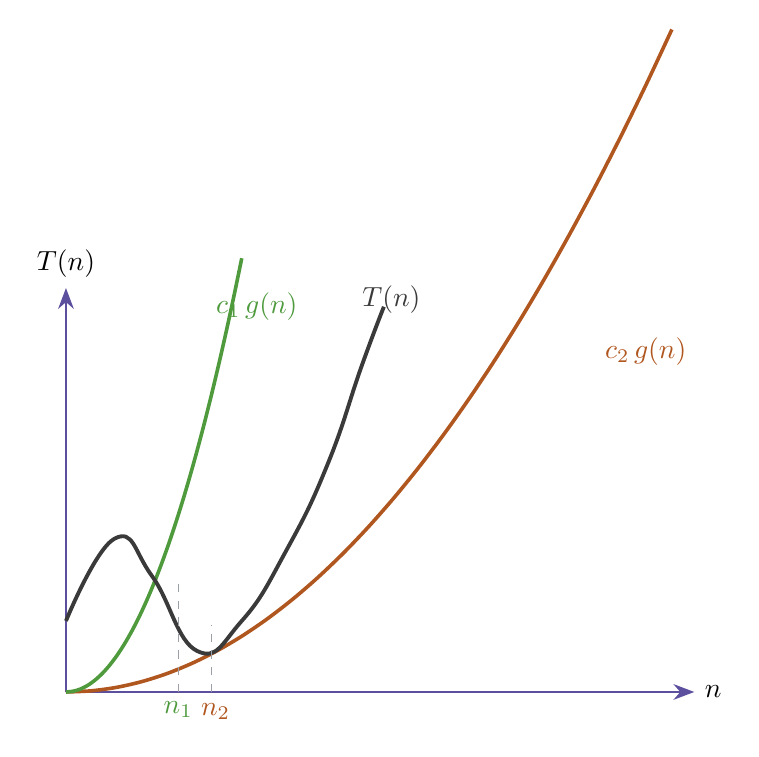
\begin{tikzpicture}[>=Stealth,scale=0.95]
  \draw[violetT,->,line width=1pt] (0,0) -- (0,5.4) node[above,black] {$T(n)$};
  \draw[violetT,->,line width=1pt] (0,0) -- (8.4,0) node[right,black] {$n$};
  \draw[rustW,line width=1.3pt,domain=0:8.1,smooth,variable=\x]
        plot ({\x},{0.135*\x*\x});
  \node[rustW] at (7.75,4.55) {$c_2\, g(n)$};
  \draw[greenO,line width=1.3pt,domain=0:2.35,smooth,variable=\x]
        plot ({\x},{1.05*\x*\x});
  \node[greenO] at (2.55,5.15) {$c_1\, g(n)$};
  \draw[inkT,line width=1.4pt,smooth,tension=0.8]
        plot coordinates {(0,0.95)(0.65,2.05)(1.15,1.55)(1.75,0.55)
                          (2.35,0.95)(2.95,1.9)(3.5,3.05)(3.95,4.35)(4.25,5.15)};
  \node[inkT] at (4.35,5.25) {$T(n)$};
  \draw[greyline,dashed] (1.5,0) -- (1.5,1.55);
  \draw[greyline,dashed] (1.95,0) -- (1.95,0.9);
  \node[greenO,below] at (1.5,0) {$n_1$};
  \node[rustW,below] at (2.0,-0.02) {$n_2$};
\end{tikzpicture}
\end{center}

Past $n_2$, $T(n)$ is trapped between the \textcolor{rustW}{$c_2 g(n)$} floor and the \textcolor{greenO}{$c_1 g(n)$} ceiling. That is $\Theta$.

% ==================================================================
\section{Worked Example: Bubble Sort is $\Theta(n^2)$}

\begin{codebox}[BubbleSort(A)]
\ttfamily for i = 1 to A.length $-$ 1:\\
\ttfamily \hspace*{2em}for j = A.length downto i + 1:\\
\ttfamily \hspace*{4em}if A[j] < A[j$-$1]: swap A[j] and A[j$-$1]
\end{codebox}

\begin{keybox}[Bubble Sort: $T(n) = \Theta(n^2)$]
\textcolor{greenO}{$O(n^2)$:} For \every{} input, the nested loops do $\sum_{i=1}^{n-1}(n-i) = \frac{n(n-1)}{2}$ comparisons. So $T(n) \le c_1 n^2$.

\textcolor{rustW}{$\Omega(n^2)$:} For \some{} input (reverse-sorted: $[n, n{-}1, \ldots, 1]$), every comparison triggers a swap, doing exactly $\frac{n(n-1)}{2}$ comparisons. So $T(n) \ge c_2 n^2$.

Same shape $\Rightarrow$ $\Theta(n^2)$.
\end{keybox}

\begin{examplebox}[Practice: is $3n^2 + 5n\log n$ in $\Theta(n^2)$?]
\textcolor{greenO}{$O(n^2)$:} $3n^2 + 5n\log n \le 3n^2 + 5n^2 = 8n^2$ for $n \ge 1$. \checkmark

\textcolor{rustW}{$\Omega(n^2)$:} $3n^2 + 5n\log n \ge 3n^2$ for $n \ge 1$. \checkmark

Yes, $3n^2 + 5n\log n = \Theta(n^2)$.
\end{examplebox}

\begin{keybox}[Quick Reference: Lecture 1]
\renewcommand{\arraystretch}{1.35}
\begin{tabular}{l l}
$T(n)$ & $\max\{t(x) \mid x \text{ of size } n\}$ \\
\textcolor{greenO}{$O(g(n))$} & $T(n) \le c\,g(n)$ eventually \quad \every{} input, \atmost \\
\textcolor{rustW}{$\Omega(g(n))$} & $T(n) \ge c\,g(n)$ eventually \quad \some{} input, \atleast \\
\textcolor{violetT}{$\Theta(g(n))$} & both $O$ and $\Omega$ with same $g$ (tight) \\
Bubble sort & $\Theta(n^2)$ \\
\end{tabular}
\end{keybox}

\newpage

% ******************************************************************
%  PART II: LECTURE 2 — PRIORITY QUEUES AND MAX-HEAPS
% ******************************************************************

\part*{\textcolor{utnavy}{Lecture 2: Priority Queues and Max-Heaps}}
\addcontentsline{toc}{part}{Lecture 2: Priority Queues and Max-Heaps}

% ==================================================================
\section{ADT vs.\ Data Structure}

\begin{defbox}[Two different things]
\textbf{Abstract data type (ADT):} specifies an \textcolor{rustW}{object} + \textcolor{rustW}{operations}. Says \emph{what}, not \emph{how}.

\textbf{Data structure:} \textcolor{rustW}{one specific implementation} of an ADT (memory layout + code for each operation).

Multiple data structures can implement the same ADT, with different costs.
\end{defbox}

% ==================================================================
\section{The Priority Queue ADT}

\begin{defbox}[Priority Queue ADT]
\textbf{Object:} a set $S$ of elements, each with a comparable \textcolor{rustW}{key} (priority).

\textbf{Operations:}
\begin{itemize}[leftmargin=1.4em,itemsep=1pt]
  \item \textbf{Insert}$(S,x)$: add element $x$ into $S$.
  \item \textbf{Max}$(S)$: return element with highest priority (no removal).
  \item \textbf{Extract\_Max}$(S)$: return \textbf{and remove} element with highest priority.
\end{itemize}
\end{defbox}

\textbf{Application:} OS job scheduling. Jobs arrive $\to$ \textbf{Insert}. Processor free $\to$ \textbf{Extract\_Max} to run the highest-priority job.

% ==================================================================
\section{Naive Implementations: Why We Need Something Better}

\begin{center}
\renewcommand{\arraystretch}{1.5}
\begin{tabular}{l c c}
\hline
\textbf{\textcolor{heapblue}{Worst case}} & \textbf{Insert} & \textbf{Extract\_Max}\\
\hline
Unordered linked list & \textcolor{greenO}{$\Theta(1)$} & \textcolor{rustW}{$\Theta(n)$}\\
Ordered linked list   & \textcolor{rustW}{$\Theta(n)$} & \textcolor{greenO}{$\Theta(1)$}\\
\hline
\end{tabular}
\end{center}

\textbf{Unordered:} Insert at front is $\Theta(1)$, but Extract\_Max scans the whole list $\Rightarrow$ $\Theta(n)$.

\textbf{Ordered:} Max is at the end $\Rightarrow$ Extract\_Max is $\Theta(1)$, but inserting in sorted position $\Rightarrow$ $\Theta(n)$.

\begin{keybox}[Goal]
Both operations in \textcolor{rustW}{$O(\log n)$}. A \textbf{max-heap} achieves this.
\end{keybox}

% ==================================================================
\section{Complete Binary Tree (CBT)}

\begin{defbox}[Complete Binary Tree]
A binary tree where:
\begin{itemize}[leftmargin=1.4em,itemsep=1pt]
  \item every level except possibly the last is completely full,
  \item the last level is filled \textcolor{rustW}{from the left} with no gaps.
\end{itemize}
\end{defbox}

\begin{center}
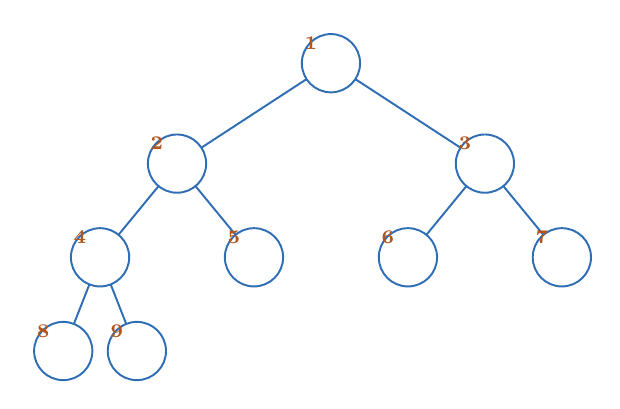
\begin{tikzpicture}[scale=0.85]
\drawheap{1//black,2//black,3//black,4//black,5//black,6//black,7//black,8//black,9//black}{1/2,1/3,2/4,2/5,3/6,3/7,4/8,4/9}
\end{tikzpicture}
\end{center}

\subsection{Height}

\begin{defbox}[Height of a tree]
Number of \textcolor{rustW}{edges} on the longest root-to-leaf path.
\end{defbox}

\begin{center}
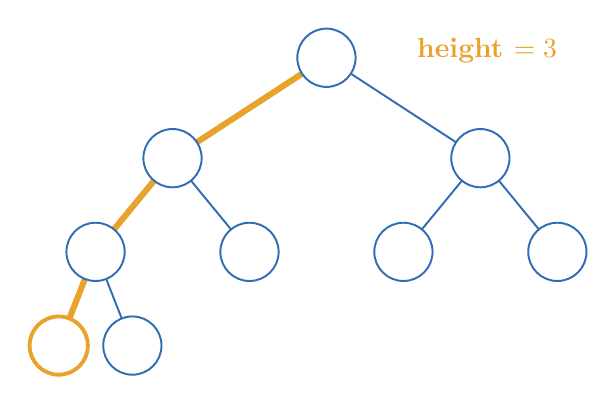
\begin{tikzpicture}[scale=0.85]
\heapcoords
\begin{scope}[on background layer]
  \foreach \a/\b in {1/3,2/5,3/6,3/7,4/9}{\draw[hedge] (p\a)--(p\b);}
  \foreach \a/\b in {1/2,2/4,4/8}{\draw[goldpath,line width=2.2pt] (p\a)--(p\b);}
\end{scope}
\foreach \idx in {1,2,3,4,5,6,7,9}{\node[hnode] at (p\idx){};}
\node[hnode,draw=goldpath,line width=1.4pt] at (p8){};
\node[goldpath,font=\bfseries] at (2.4,4.6){height $=3$};
\end{tikzpicture}
\end{center}

\begin{keybox}[Key fact]
A CBT with $n$ nodes has height $\lfloor \log_2 n \rfloor$.

Each full level doubles the node count ($1, 2, 4, 8, \ldots$), so $\log_2 n$ levels suffice for $n$ nodes.
\end{keybox}

% ==================================================================
\section{Max-Heap}

\begin{defbox}[Max-Heap = CBT + max-heap property]
Elements stored in a CBT such that:
\begin{center}\large
priority(node) $\;\textcolor{rustW}{\ge}\;$ priority(each child)
\end{center}
This is a \textbf{local} rule (parent vs.\ own children only). It chains upward, so the \textbf{global max is always at the root}.
\end{defbox}

\subsection*{Example}
$S=\{3,4,5,7,7,9,9,12,17\}$. One valid max-heap:

\begin{center}
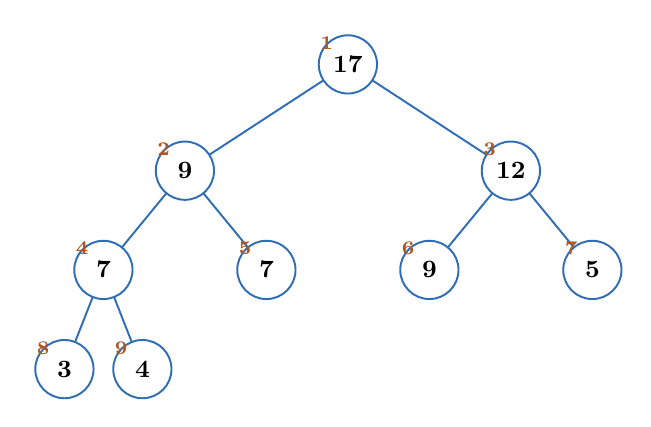
\begin{tikzpicture}[scale=0.9]
\drawheap{1/17/black,2/9/black,3/12/black,4/7/black,5/7/black,6/9/black,7/5/black,8/3/black,9/4/black}{1/2,1/3,2/4,2/5,3/6,3/7,4/8,4/9}
\end{tikzpicture}
\end{center}

Check: $17 \ge 9, 12$. \; $9 \ge 7, 7$. \; $12 \ge 9, 5$. \checkmark

Swapping children of the root ($9 \leftrightarrow 12$) gives a different valid heap $\Rightarrow$ \textcolor{rustW}{max-heaps are not unique}. Only the root (global max) is guaranteed.

% ==================================================================
\section{Array Representation}

Store the tree \textbf{level by level, left to right} in array \texttt{A[1..n]}. No pointers needed.

\begin{center}
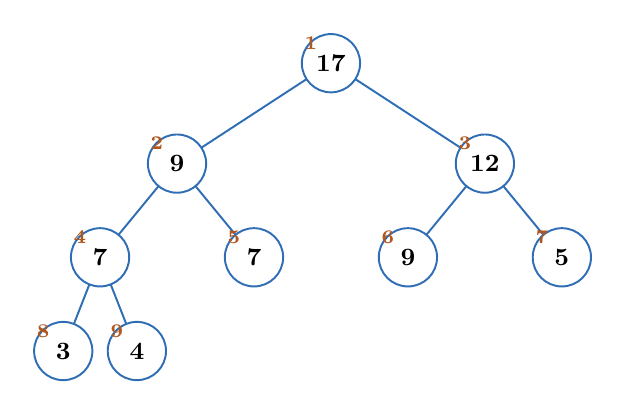
\begin{tikzpicture}[scale=0.85]
\drawheap{1/17/black,2/9/black,3/12/black,4/7/black,5/7/black,6/9/black,7/5/black,8/3/black,9/4/black}{1/2,1/3,2/4,2/5,3/6,3/7,4/8,4/9}
\end{tikzpicture}\\[8pt]
\heaparray{17,9,12,7,7,9,5,3,4}
\end{center}

\begin{keybox}[Navigation formulas]
For node at index $i$:
\begin{itemize}[leftmargin=1.4em,itemsep=1pt]
  \item \textbf{Left child:} $2i$ \qquad \textbf{Right child:} $2i+1$ \qquad \textbf{Parent:} $\lfloor i/2 \rfloor$
\end{itemize}
\texttt{A.heapsize} tracks the number of elements currently in the heap.
\end{keybox}

\begin{examplebox}[Verify: node at $i=2$ holds $9$]
Left child: $A[2 \cdot 2] = A[4] = 7$ \checkmark \quad Right child: $A[2 \cdot 2 + 1] = A[5] = 7$ \checkmark

Parent: $A[\lfloor 2/2 \rfloor] = A[1] = 17$ \checkmark

Each level is $\sim 2\times$ the width of the one above, so going down doubles the index, going up halves it.
\end{examplebox}

% ==================================================================
\section{The Three Operations}

\begin{keybox}[Invariant for every operation]
1) Maintain the \textcolor{rustW}{CBT shape}. \quad 2) Maintain the \textcolor{rustW}{max-heap property}.
\end{keybox}

\subsection{Max(A)}

\begin{codebox}[Max(A)]
\ttfamily return A[1]
\end{codebox}

The root always holds the max. $\Rightarrow$ \textcolor{greenO}{$\Theta(1)$}.

\subsection{Insert(A, x): percolate up}

\begin{codebox}[Insert(A, x)]
\ttfamily 1. A.heapsize++; A[A.heapsize] = x \hfill\textnormal{\itshape (place at next open leaf)}\\[3pt]
\ttfamily 2. while x is not root and priority(x) > priority(parent(x)):\\
\ttfamily \hspace*{2em}swap x with parent(x) \hfill\textnormal{\itshape (percolate up)}
\end{codebox}

\subsubsection*{Worked example: Insert(A, 13)}
Start: $A = [17,9,12,7,7,9,5,3,4]$. Insert $13$ at index $10$.

\textbf{Step 1.} Place $13$ at $A[10]$. Property broken: $13 > 7$ (parent at $i=5$).

\begin{center}
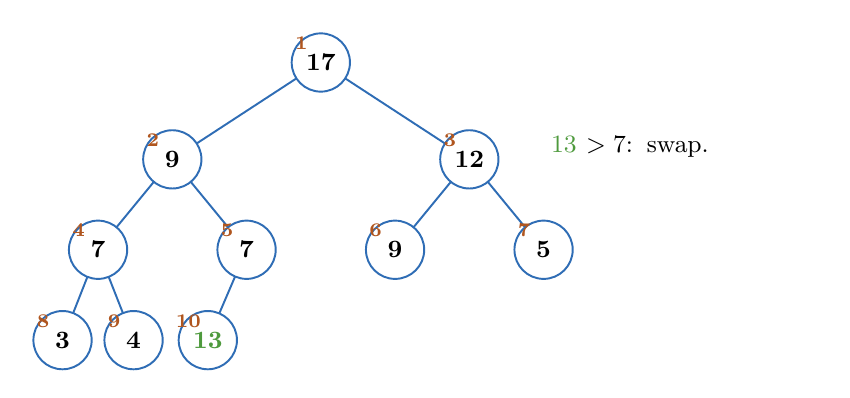
\begin{tikzpicture}[scale=0.82]
\drawheap{1/17/black,2/9/black,3/12/black,4/7/black,5/7/black,6/9/black,7/5/black,8/3/black,9/4/black,10/13/greenO}{1/2,1/3,2/4,2/5,3/6,3/7,4/8,4/9,5/10}
\node[align=left,text width=3.3cm] at (5.6,3.2){\small \textcolor{greenO}{$13$} $> 7$: swap.};
\end{tikzpicture}
\end{center}

\textbf{Step 2a.} Swap $13 \leftrightarrow 7$. Now $13$ at $i=5$. Compare: $13 > 9$ (parent at $i=2$).

\begin{center}
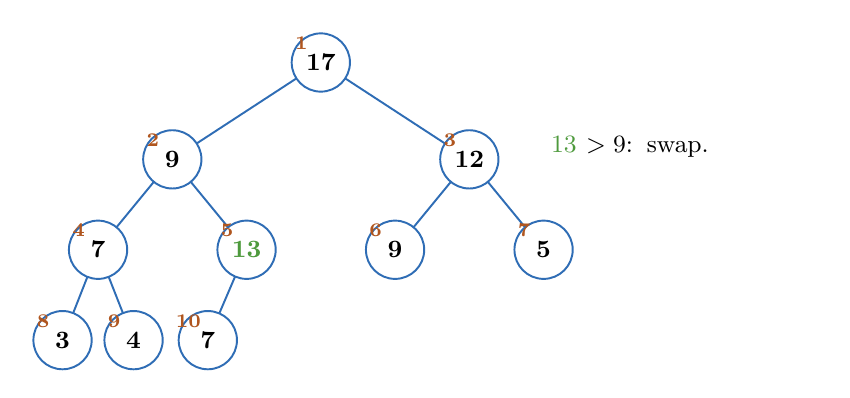
\begin{tikzpicture}[scale=0.82]
\drawheap{1/17/black,2/9/black,3/12/black,4/7/black,5/13/greenO,6/9/black,7/5/black,8/3/black,9/4/black,10/7/black}{1/2,1/3,2/4,2/5,3/6,3/7,4/8,4/9,5/10}
\node[align=left,text width=3.3cm] at (5.6,3.2){\small \textcolor{greenO}{$13$} $> 9$: swap.};
\end{tikzpicture}
\end{center}

\textbf{Step 2b.} Swap $13 \leftrightarrow 9$. Now $13$ at $i=2$. Compare: $13 < 17$ (root). Stop.

\begin{center}
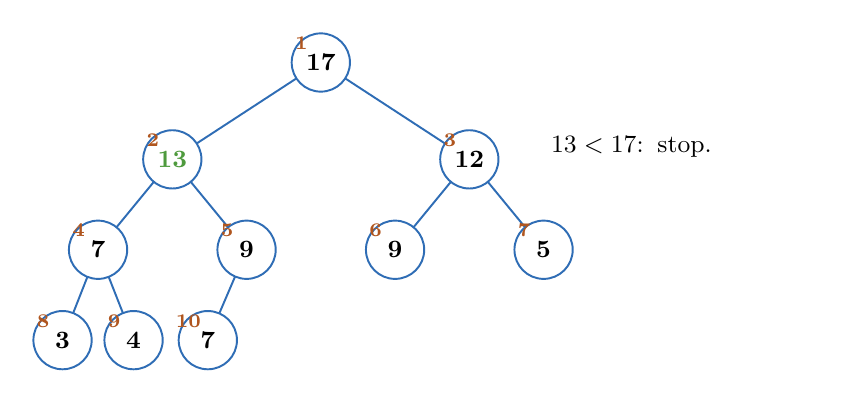
\begin{tikzpicture}[scale=0.82]
\drawheap{1/17/black,2/13/greenO,3/12/black,4/7/black,5/9/black,6/9/black,7/5/black,8/3/black,9/4/black,10/7/black}{1/2,1/3,2/4,2/5,3/6,3/7,4/8,4/9,5/10}
\node[align=left,text width=3.3cm] at (5.6,3.2){\small $13 < 17$: stop.};
\end{tikzpicture}
\end{center}

Result: $A = [17,13,12,7,9,9,5,3,4,7]$, \texttt{heapsize}$=10$.

\subsection{Extract\_Max(A): drip down}

\begin{codebox}[Extract\_Max(A)]
\ttfamily 1. max = A[1] \hfill\textnormal{\itshape (save the root)}\\[3pt]
\ttfamily 2. A[1] = A[A.heapsize]; A.heapsize{-}{-} \hfill\textnormal{\itshape (move last leaf to root)}\\[3pt]
\ttfamily 3. while x has a child with higher priority:\\
\ttfamily \hspace*{2em}swap x with its \textbf{largest} child \hfill\textnormal{\itshape (drip down)}\\[3pt]
\ttfamily 4. return max
\end{codebox}

Important: always swap with the \emph{larger} child (otherwise we create a new violation). Node at index $i$ is a leaf when $i > \lfloor \texttt{heapsize}/2 \rfloor$.

\subsubsection*{Worked example: Extract\_Max(A)}
Start: $A = [17,13,12,7,9,9,5,3,4,7]$, \texttt{heapsize}$=10$.

\textbf{Steps 1\,\&\,2.} Save $17$. Move $A[10]=7$ to root. Shrink \texttt{heapsize} to $9$.

\begin{center}
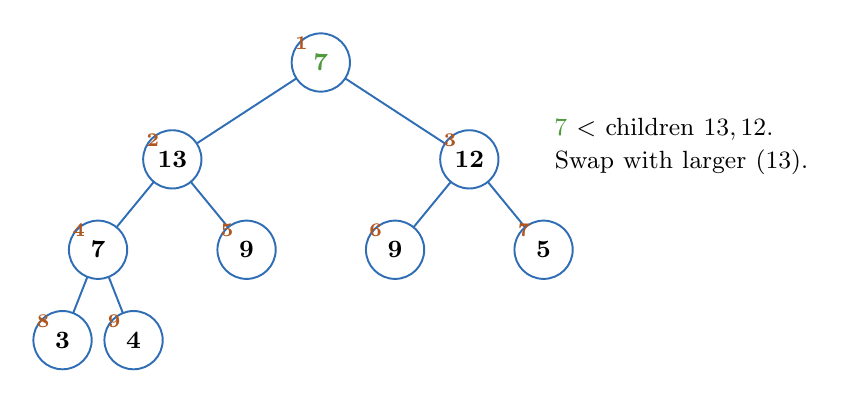
\begin{tikzpicture}[scale=0.82]
\drawheap{1/7/greenO,2/13/black,3/12/black,4/7/black,5/9/black,6/9/black,7/5/black,8/3/black,9/4/black}{1/2,1/3,2/4,2/5,3/6,3/7,4/8,4/9}
\node[align=left,text width=3.4cm] at (5.7,3.2){\small \textcolor{greenO}{$7$} $<$ children $13, 12$. Swap with larger ($13$).};
\end{tikzpicture}
\end{center}

\textbf{Step 3a.} Swap $7 \leftrightarrow 13$. Now $7$ at $i=2$. Children: $7, 9$. Larger is $9 > 7$.

\begin{center}
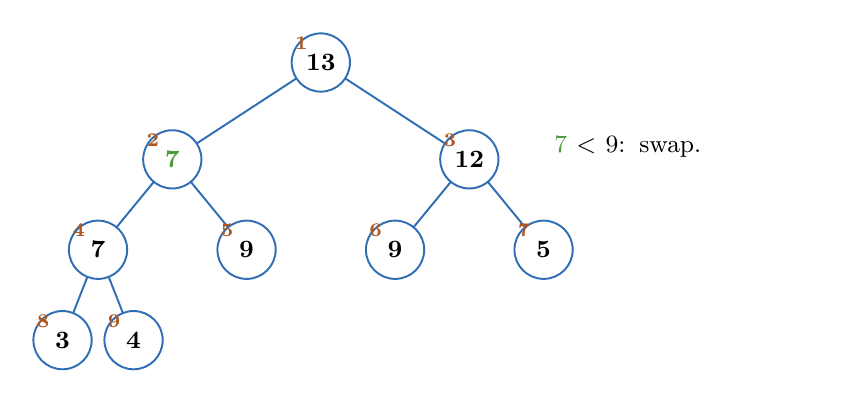
\begin{tikzpicture}[scale=0.82]
\drawheap{1/13/black,2/7/greenO,3/12/black,4/7/black,5/9/black,6/9/black,7/5/black,8/3/black,9/4/black}{1/2,1/3,2/4,2/5,3/6,3/7,4/8,4/9}
\node[align=left,text width=3.4cm] at (5.7,3.2){\small \textcolor{greenO}{$7$} $<$ $9$: swap.};
\end{tikzpicture}
\end{center}

\textbf{Step 3b.} Swap $7 \leftrightarrow 9$. Now $7$ at $i=5$. Children at $i=10 >$ \texttt{heapsize}$=9$, so $7$ is a leaf. Stop.

\begin{center}
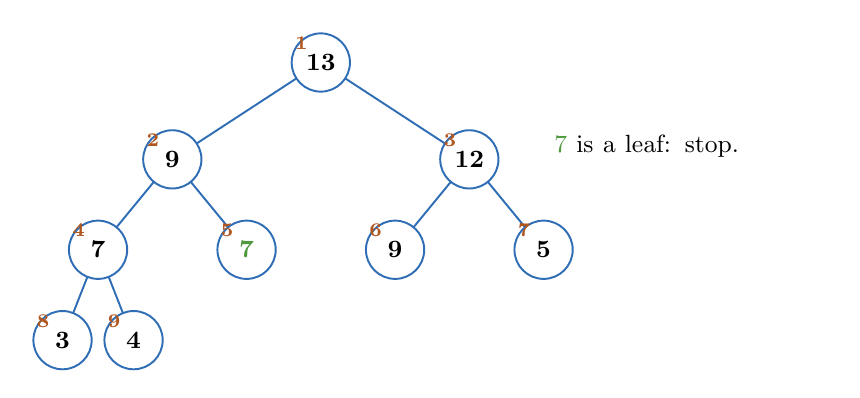
\begin{tikzpicture}[scale=0.82]
\drawheap{1/13/black,2/9/black,3/12/black,4/7/black,5/7/greenO,6/9/black,7/5/black,8/3/black,9/4/black}{1/2,1/3,2/4,2/5,3/6,3/7,4/8,4/9}
\node[align=left,text width=3.4cm] at (5.7,3.2){\small \textcolor{greenO}{$7$} is a leaf: stop.};
\end{tikzpicture}
\end{center}

Return $17$. Heap: $[13,9,12,7,7,9,5,3,4]$.

% ==================================================================
\section{Complexity Analysis}

Each operation walks one root-to-leaf (or leaf-to-root) path. Path length $\le$ height $= \lfloor \log_2 n \rfloor$. Constant work per level.

\begin{keybox}[Heap operation costs]
\renewcommand{\arraystretch}{1.4}
\begin{tabular}{l l l}
\textbf{Max}$(A)$ & \textcolor{greenO}{$\Theta(1)$} & read root\\
\textbf{Insert}$(A,x)$ & \textcolor{violetT}{$\Theta(\log n)$} & percolate up $\le \lfloor\log_2 n\rfloor$ levels\\
\textbf{Extract\_Max}$(A)$ & \textcolor{violetT}{$\Theta(\log n)$} & drip down $\le \lfloor\log_2 n\rfloor$ levels\\
\end{tabular}
\end{keybox}

\textbf{Insert} $= \Theta(\log n)$:
\begin{itemize}[leftmargin=1.4em,itemsep=2pt]
  \item \textcolor{greenO}{$O(\log n)$:} At most $\lfloor\log_2 n\rfloor$ swaps (one per level). \every{} input, \atmost{} $c_1 \log n$.
  \item \textcolor{rustW}{$\Omega(\log n)$:} Insert a value larger than the current root $\Rightarrow$ percolates all the way to the top. \some{} input, \atleast{} $c_2 \log n$.
\end{itemize}

Same argument for Extract\_Max (drip down with the smallest value $\Rightarrow$ sinks to a leaf).

% ==================================================================
\section{HeapSort}

\begin{keybox}[HeapSort]
\begin{enumerate}[leftmargin=1.6em,itemsep=2pt]
  \item Build a max-heap from $A$. \quad{\small($\Theta(n)$ time)}
  \item Call \textbf{Extract\_Max} $n$ times. \quad{\small(each $\Theta(\log n)$)}
\end{enumerate}
\[
  \text{Total: } n \times \Theta(\log n) = \textcolor{violetT}{\Theta(n \log n)}
\]
\end{keybox}

\begin{center}
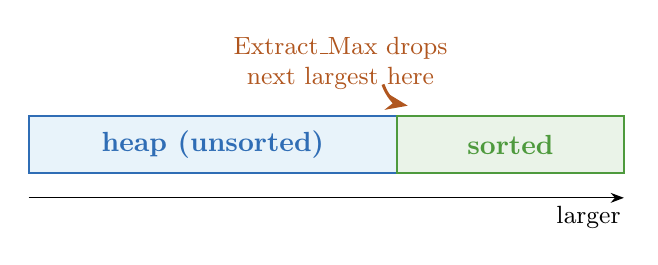
\begin{tikzpicture}[scale=0.9]
\draw[fill=skyfill,draw=heapblue,line width=0.7pt] (0,0) rectangle (5.2,0.8);
\draw[fill=greenO!12,draw=greenO,line width=0.7pt] (5.2,0) rectangle (8.4,0.8);
\node[heapblue,font=\bfseries] at (2.6,0.4){heap (unsorted)};
\node[greenO,font=\bfseries] at (6.8,0.4){sorted};
\draw[-{Stealth},line width=1.1pt,rustW] (5.0,1.25) to[bend right=30] (5.35,0.95);
\node[rustW,font=\small,align=center] at (4.4,1.55){Extract\_Max drops\\next largest here};
\draw[-{Stealth}] (0,-0.35)--(8.4,-0.35);
\node[font=\small] at (7.9,-0.62){larger};
\end{tikzpicture}
\end{center}

Each extraction moves the max to the front of the sorted region. The heap shrinks by one, the sorted region grows by one. After $n$ extractions, the array is sorted in place.

% ==================================================================
\section{Past Exam: $k$-Set ADT}

\begin{exambox}[Seen on a past exam \textnormal{(Midterm, Fall 2014, Q2)}]
The \emph{rank} of an element = its position in sorted order (from $1$). For fixed $k \in \mathbb{Z}^+$:
\begin{itemize}[leftmargin=1.4em,itemsep=1pt]
  \item \textbf{Object:} collection $C$ of rationals (duplicates allowed).
  \item \textbf{Insert}$(C,x)$: add $x$ to $C$.
  \item \textbf{$k$-Select}$(C)$: return element at rank $k$, or \texttt{nil} if $|C| < k$.
\end{itemize}
\textbf{Q.} Implement with data structures from class. \textbf{$k$-Select} must be $O(1)$.

\begin{answerband}
\textbf{Data structure:} \textbf{max-heap} $H_1$ (stores the $k$ smallest elements) + \textbf{min-heap} $H_2$ (stores the rest).

The $k$-th smallest element = the largest among the $k$ smallest = root of $H_1$.

\smallskip
\textbf{$k$-Select$(C)$:}\\
\hspace*{1.5em}\texttt{if $|H_1| < k$: return nil}\\
\hspace*{1.5em}\texttt{else: return $H_1[1]$} \hfill $\Rightarrow$ \textcolor{greenO}{$O(1)$}

\smallskip
\textbf{Insert$(C,x)$:}\\
\hspace*{1.5em}\texttt{if $|H_1| < k$ or $x < H_1[1]$: insert $x$ into $H_1$}\\
\hspace*{1.5em}\texttt{else: insert $x$ into $H_2$}\\
\hspace*{1.5em}\texttt{if $|H_1| > k$: insert Extract-Max($H_1$) into $H_2$}\\
Constant number of heap ops, each $O(\log n)$ $\Rightarrow$ \textcolor{violetT}{$O(\log n)$}.

\smallskip
\textbf{Correctness:} $H_1$ always holds exactly the $k$ smallest. New small values enter $H_1$; overflow gets pushed to $H_2$. Large values go straight to $H_2$.
\end{answerband}
\end{exambox}

% ==================================================================
\section*{\textcolor{violetT}{Quick Reference: Lecture 2}}
\addcontentsline{toc}{section}{Quick Reference: Lecture 2}
\begin{keybox}
\renewcommand{\arraystretch}{1.35}
\begin{tabular}{l l}
Max-heap property & priority(node) $\ge$ priority(children); max at root \texttt{A[1]}\\
Array navigation & left $=2i$, \; right $=2i+1$, \; parent $=\lfloor i/2\rfloor$\\
Height of CBT & $\lfloor \log_2 n \rfloor$\\
\textbf{Max} & read \texttt{A[1]} $\to$ \textcolor{greenO}{$\Theta(1)$}\\
\textbf{Insert} & place at end, percolate up $\to$ \textcolor{violetT}{$\Theta(\log n)$}\\
\textbf{Extract\_Max} & move last to root, drip down $\to$ \textcolor{violetT}{$\Theta(\log n)$}\\
\textbf{HeapSort} & build heap + $n$ extractions $\to$ \textcolor{violetT}{$\Theta(n\log n)$}\\
\end{tabular}
\end{keybox}

\vspace{4pt}
\begin{center}\textcolor{greyline}{\rule{0.5\linewidth}{0.6pt}}\end{center}



\newpage
 


% ******************************************************************
%  PASTE INSTRUCTIONS:
%
%  1. In your master document, DELETE these 3 lines near the end:
%       \begin{center}\textcolor{greyline}{\rule{0.5\linewidth}{0.6pt}}\end{center}
%       
%       \end{document}
%
%  2. Paste EVERYTHING below this comment block in their place.
%
%  3. On the cover page, change:
%       {\large\textcolor{violetT}{Lectures 1, 2, 3 \& 4}}
%     to:
%       {\large\textcolor{violetT}{Lectures 1, 2 \& 3}}
%
%  That's it. No preamble changes needed.
% ******************************************************************

\newpage

% ******************************************************************
%  PART III: LECTURE 3 — MIN BINOMIAL HEAPS
% ******************************************************************

\part*{\textcolor{utnavy}{Lecture 3: Min Binomial Heaps}}
\addcontentsline{toc}{part}{Lecture 3: Min Binomial Heaps}

% ==================================================================
\section{Mergeable Priority Queue ADT}

Last lecture: Priority Queue ADT (Insert, Max, Extract\_Max). Now we flip to \textbf{min} (smallest key = highest priority) and add one more operation:

\begin{defbox}[Mergeable Priority Queue ADT]
\textbf{Object:} a set $S$ of elements, each with a comparable \textcolor{rustW}{key}.

\textbf{Operations:}
\begin{itemize}[leftmargin=1.4em,itemsep=1pt]
  \item \textbf{Insert}$(S, x)$: add element $x$ to $S$.
  \item \textbf{Min}$(S)$: return the element with the smallest key.
  \item \textbf{Extract\_Min}$(S)$: remove and return the element with the smallest key.
  \item \textbf{Union}$(S_1, S_2)$: merge two priority queues into a single one.
\end{itemize}
\end{defbox}

\begin{center}
\renewcommand{\arraystretch}{1.5}
\begin{tabular}{l c c}
\hline
\textbf{\textcolor{heapblue}{Operation}} & \textbf{Min Heap (array)} & \textbf{Min Binomial Heap}\\
\hline
\texttt{Insert} & $O(\log n)$ & $O(\log n)$\\
\texttt{Min} & \textcolor{greenO}{$O(1)$} & $O(\log n)$\\
\texttt{Extract\_Min} & $O(\log n)$ & $O(\log n)$\\
\texttt{Union} & \textcolor{rustW}{$O(n)$} & \textcolor{greenO}{$O(\log n)$}\\
\hline
\end{tabular}
\end{center}

\begin{warnbox}[Why regular min heaps fail at Union]
A binary min heap stores elements in an array. To merge two heaps you basically dump them together and rebuild. That costs $O(n)$. Binomial heaps are specifically \textbf{designed} so Union runs in $\textcolor{greenO}{O(\log n)}$.
\end{warnbox}

% ==================================================================
\section{Binomial Trees}

\subsection{Recursive Definition of $B_k$}

\begin{defbox}[Binomial Tree $B_k$]
\textbf{Base case:} $B_0$ = a single node.\\[4pt]
\textbf{Recursive case:} $B_k$ = take two copies of $B_{k-1}$. Make one root the \textbf{leftmost child} of the other root.\\[6pt]
Equivalently: the root of $B_k$ has children $B_{k-1},\, B_{k-2},\, \ldots,\, B_1,\, B_0$ (left to right).
\end{defbox}

\begin{keybox}[Breaking Down the Recursive Definition]
This is a common confusion point, so let's be explicit.

To build $B_k$:
\begin{enumerate}[leftmargin=1.4em,itemsep=2pt]
  \item Start with one copy of $B_{k-1}$. Call its root $r$.
  \item Take a \textbf{second} copy of $B_{k-1}$.
  \item Make the root of copy 2 the \textbf{new overall root}, and attach $r$'s entire tree as a subtree under it.
\end{enumerate}

So $B_k$ = \textbf{two $B_{k-1}$'s glued together}, one becoming a child of the other.
\end{keybox}

\subsubsection*{Building Up From $B_0$}

\begin{center}
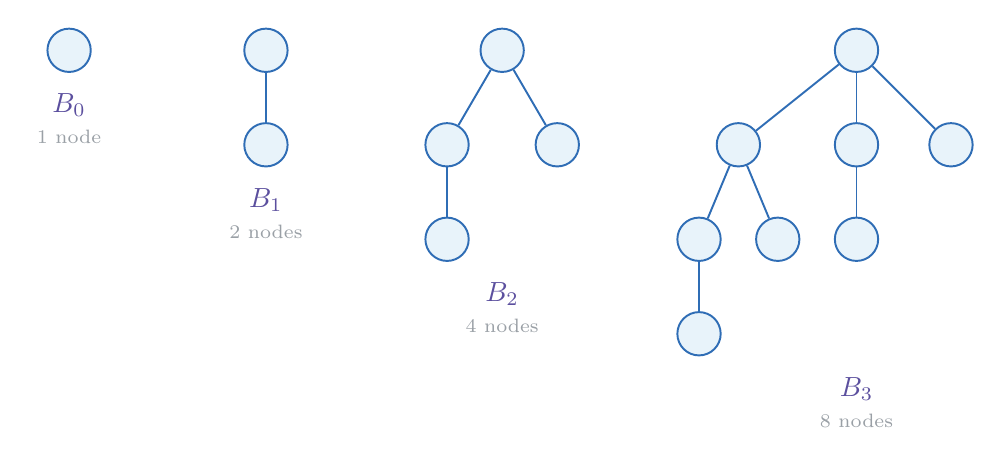
\begin{tikzpicture}[
  bnode/.style={circle, draw=heapblue, line width=0.7pt, minimum size=5.5mm, inner sep=0pt, fill=skyfill},
]
% B_0
\node[bnode] (a0) at (0,0) {};
\node[font=\bfseries\color{violetT}] at (0,-0.7) {$B_0$};
\node[font=\scriptsize\color{greyline}] at (0,-1.1) {1 node};

% B_1
\node[bnode] (b0) at (2.5,0) {};
\node[bnode] (b1) at (2.5,-1.2) {};
\draw[heapblue, line width=0.7pt] (b0) -- (b1);
\node[font=\bfseries\color{violetT}] at (2.5,-1.9) {$B_1$};
\node[font=\scriptsize\color{greyline}] at (2.5,-2.3) {2 nodes};

% B_2
\node[bnode] (c0) at (5.5,0) {};
\node[bnode] (c1) at (4.8,-1.2) {};
\node[bnode] (c2) at (6.2,-1.2) {};
\node[bnode] (c3) at (4.8,-2.4) {};
\draw[heapblue, line width=0.7pt] (c0) -- (c1);
\draw[heapblue, line width=0.7pt] (c0) -- (c2);
\draw[heapblue, line width=0.7pt] (c1) -- (c3);
\node[font=\bfseries\color{violetT}] at (5.5,-3.1) {$B_2$};
\node[font=\scriptsize\color{greyline}] at (5.5,-3.5) {4 nodes};

% B_3
\node[bnode] (d0) at (10,0) {};
\node[bnode] (d1) at (8.5,-1.2) {};
\node[bnode] (d2) at (10,-1.2) {};
\node[bnode] (d3) at (11.2,-1.2) {};
\node[bnode] (d4) at (8,-2.4) {};
\node[bnode] (d5) at (9,-2.4) {};
\node[bnode] (d6) at (10,-2.4) {};
\node[bnode] (d7) at (8,-3.6) {};
\draw[heapblue, line width=0.7pt] (d0) -- (d1);
\draw[heapblue, line width=0.7pt] (d0) -- (d2);
\draw[heapblue, line width=0.7pt] (d0) -- (d3);
\draw[heapblue, line width=0.7pt] (d1) -- (d4);
\draw[heapblue, line width=0.7pt] (d1) -- (d5);
\draw[heapblue, line width=0.7pt] (d2) -- (d6);
\draw[heapblue, line width=0.7pt] (d4) -- (d7);
\node[font=\bfseries\color{violetT}] at (10,-4.3) {$B_3$};
\node[font=\scriptsize\color{greyline}] at (10,-4.7) {8 nodes};
\end{tikzpicture}
\end{center}

\subsection{Children Sequence of $B_k$}

\begin{keybox}[Children of the Root of $B_k$]
The root of $B_k$ has exactly $k$ children. Reading \textbf{left to right}:
$$\underbrace{B_{k-1}}_{\text{leftmost (biggest)}},\; B_{k-2},\; \ldots,\; B_1,\; \underbrace{B_0}_{\text{rightmost (single node)}}$$

The \textcolor{rustW}{leftmost} child is the \textcolor{rustW}{largest} subtree ($B_{k-1}$), and the \textcolor{greenO}{rightmost} child is the \textcolor{greenO}{smallest} ($B_0$).

This ordering matters a lot for the memory representation later.
\end{keybox}

\begin{examplebox}[Visualizing $B_4$: Children of the Root]
The \textcolor{rustW}{root} of $B_4$ has children $B_3, B_2, B_1, B_0$ (left to right, largest subtree to smallest). Total: $2^4 = 16$ nodes, height 4.

\begin{center}
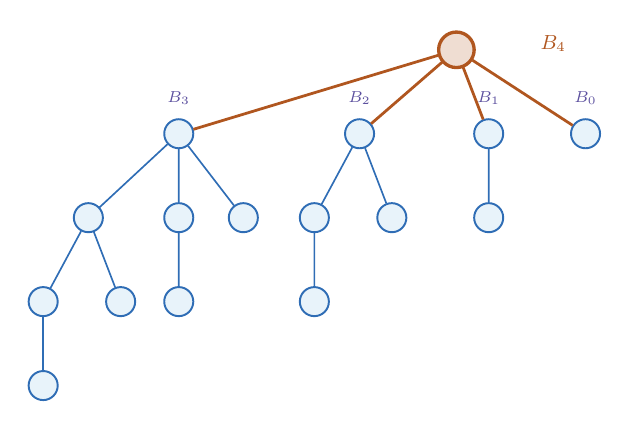
\begin{tikzpicture}[
  bnode/.style={circle, draw=heapblue, line width=0.7pt, minimum size=4.5mm, inner sep=0pt, fill=skyfill},
  rnode/.style={circle, draw=rustW, line width=1.2pt, minimum size=5.5mm, inner sep=0pt, fill=rustW!20},
  scale=0.82, transform shape
]
% Level 0 (root)
\node[rnode] (r) at (5.5,0) {};
\node[font=\small\bfseries\color{rustW}] at (7,0.1) {$B_4$};

% Level 1: 4 children
\node[bnode] (a) at (1.2,-1.3) {};
\node[bnode] (b) at (4,-1.3) {};
\node[bnode] (c) at (6,-1.3) {};
\node[bnode] (d) at (7.5,-1.3) {};
\draw[rustW, line width=1pt] (r)--(a); \draw[rustW, line width=1pt] (r)--(b);
\draw[rustW, line width=1pt] (r)--(c); \draw[rustW, line width=1pt] (r)--(d);

% B_3 subtree (under a): 3 children
\node[bnode] (a1) at (-0.2,-2.6) {};
\node[bnode] (a2) at (1.2,-2.6) {};
\node[bnode] (a3) at (2.2,-2.6) {};
\draw[heapblue,line width=0.6pt] (a)--(a1); \draw[heapblue,line width=0.6pt] (a)--(a2);
\draw[heapblue,line width=0.6pt] (a)--(a3);
% Level 3 of B_3
\node[bnode] (a11) at (-0.9,-3.9) {};
\node[bnode] (a12) at (0.3,-3.9) {};
\node[bnode] (a21) at (1.2,-3.9) {};
\draw[heapblue,line width=0.6pt] (a1)--(a11); \draw[heapblue,line width=0.6pt] (a1)--(a12);
\draw[heapblue,line width=0.6pt] (a2)--(a21);
% Level 4 of B_3
\node[bnode] (a111) at (-0.9,-5.2) {};
\draw[heapblue,line width=0.6pt] (a11)--(a111);

% B_2 subtree (under b): 2 children
\node[bnode] (b1) at (3.3,-2.6) {};
\node[bnode] (b2) at (4.5,-2.6) {};
\draw[heapblue,line width=0.6pt] (b)--(b1); \draw[heapblue,line width=0.6pt] (b)--(b2);
\node[bnode] (b11) at (3.3,-3.9) {};
\draw[heapblue,line width=0.6pt] (b1)--(b11);

% B_1 subtree (under c): 1 child
\node[bnode] (c1) at (6,-2.6) {};
\draw[heapblue,line width=0.6pt] (c)--(c1);

% Subtree labels
\node[font=\scriptsize\bfseries\color{violetT}] at (1.2,-0.75) {$B_3$};
\node[font=\scriptsize\bfseries\color{violetT}] at (4,-0.75) {$B_2$};
\node[font=\scriptsize\bfseries\color{violetT}] at (6,-0.75) {$B_1$};
\node[font=\scriptsize\bfseries\color{violetT}] at (7.5,-0.75) {$B_0$};
\end{tikzpicture}
\end{center}
\end{examplebox}

\subsection{Properties of $B_k$}

\begin{keybox}[Key Properties of $B_k$]
\renewcommand{\arraystretch}{1.5}
\begin{tabular}{l l}
\textbf{\textcolor{violetT}{Height}} of $B_k$ & $= k$ \\
\textbf{\textcolor{violetT}{Number of nodes}} in $B_k$ & $= 2^k$ \\
\textbf{\textcolor{violetT}{Nodes at depth $d$}} in $B_k$ & $= \displaystyle\binom{k}{d}$ \\
\textbf{\textcolor{violetT}{Degree}} of root of $B_k$ & $= k$ \\
\end{tabular}
\end{keybox}

\subsection{Why ``Binomial''?}

\begin{examplebox}[Why the Name ``Binomial'']
The number of nodes at depth $d$ in $B_k$ is $\binom{k}{d}$, the \textbf{binomial coefficient} (same ``$n$ choose $k$'' from combinatorics).

Quick check for $B_3$ (8 nodes total):

\begin{center}
\renewcommand{\arraystretch}{1.3}
\begin{tabular}{l c l}
Depth 0: & $\binom{3}{0} = 1$ & (the root)\\
Depth 1: & $\binom{3}{1} = 3$ & \\
Depth 2: & $\binom{3}{2} = 3$ & \\
Depth 3: & $\binom{3}{3} = 1$ & \\
\end{tabular}
\end{center}
Total: $1 + 3 + 3 + 1 = 8$ \checkmark
\end{examplebox}

% ==================================================================
\section{Binomial Forest $F_n$}

\begin{defbox}[Binomial Forest $F_n$]
A \textbf{Binomial Forest} $F_n$ is a sequence of binomial trees $\langle B_{k_1}, B_{k_2}, \ldots, B_{k_m} \rangle$ where:
\begin{itemize}[leftmargin=1.4em,itemsep=1pt]
  \item The $k_i$ values are \textbf{strictly decreasing}: $k_1 > k_2 > \cdots > k_m$
  \item The total number of nodes across all trees $= n$
\end{itemize}
\end{defbox}

\subsection{Connection to Binary Representation}

\begin{keybox}[Binary Representation $\Leftrightarrow$ Which Trees Are Present]
Write $n$ in binary. $B_i$ is present in $F_n$ \textbf{if and only if} bit $i$ (counting from the right, starting at 0) is \textbf{1}.

This is one of the most important ideas in this lecture. The entire structure of a binomial heap is dictated by the binary representation of $n$.
\end{keybox}

\begin{examplebox}[Example: $F_7$ and $F_9$]
\textbf{$F_7$:} \quad $7 = \langle 111 \rangle_2$

All three bits are 1, so $F_7 = \langle B_2, B_1, B_0 \rangle$.

Sizes: $4 + 2 + 1 = 7$ \checkmark \\[6pt]

\textbf{$F_9$:} \quad $9 = \langle 1001 \rangle_2$

Bits 0 and 3 are 1, so $F_9 = \langle B_3, B_0 \rangle$.

Sizes: $8 + 1 = 9$ \checkmark
\end{examplebox}

\subsection{What is $\alpha(n)$?}

\begin{defbox}[$\alpha(n)$ (popcount)]
$\alpha(n)$ = the number of \textbf{1's} in the binary representation of $n$.

Other names: \textbf{popcount}, \textbf{Hamming weight}, \textbf{bit population count}.
\end{defbox}

\begin{examplebox}[Computing $\alpha(n)$]
\begin{center}
\renewcommand{\arraystretch}{1.3}
\begin{tabular}{l l l}
$\alpha(7)$ & $= \alpha(\langle 111 \rangle_2)$ & $= 3$ \\
$\alpha(9)$ & $= \alpha(\langle 1001 \rangle_2)$ & $= 2$ \\
$\alpha(16)$ & $= \alpha(\langle 10000 \rangle_2)$ & $= 1$ \\
$\alpha(15)$ & $= \alpha(\langle 1111 \rangle_2)$ & $= 4$ \\
\end{tabular}
\end{center}
\end{examplebox}

\subsection{Properties of $F_n$}

\begin{keybox}[Properties of $F_n$]
\renewcommand{\arraystretch}{1.5}
\begin{tabular}{l l}
Number of trees in $F_n$ & $= \textcolor{violetT}{\alpha(n)}$ \quad (one per 1 bit) \\
Max number of trees & $\le \lfloor \log_2 n \rfloor + 1$ \\
Number of edges in $F_n$ & $= \textcolor{violetT}{n - \alpha(n)}$ \\
\end{tabular}
\end{keybox}

\begin{examplebox}[Verifying Edge Count for $F_7$]
$F_7 = \langle B_2, B_1, B_0 \rangle$.

Edges in $B_2$: 3, \quad edges in $B_1$: 1, \quad edges in $B_0$: 0. \quad Total = 4.

Formula: $n - \alpha(n) = 7 - 3 = 4$ \checkmark
\end{examplebox}

% ==================================================================
\section{Min Binomial Heap: The Full Definition}

\begin{defbox}[Min Binomial Heap]
A \textbf{Min Binomial Heap} of $n$ elements is a Binomial Forest $F_n$ such that:
\begin{enumerate}[leftmargin=1.4em,itemsep=3pt]
  \item \textcolor{defblue}{\textbf{One element per node:}} each node stores exactly one element.
  \item \textcolor{defblue}{\textbf{Min heap ordering:}} in each tree, every node's key $\le$ all keys in its subtree. (Root of each tree = smallest key in that tree.)
\end{enumerate}
\end{defbox}

\begin{warnbox}[It's a forest, not a single tree!]
A Min Binomial Heap is a \textbf{collection of trees} (a forest). Each individual tree is a binomial tree satisfying the min heap property. Do not confuse this with a single binary heap.
\end{warnbox}

% ==================================================================
\section{Building a Binomial Heap: Worked Example}

\begin{examplebox}[Build a Min Binomial Heap from $S = \{10, 13, 1, 3, 8, 18, 7\}$]
$n = 7$, and $7 = \langle 111 \rangle_2$, so the final forest = $\langle B_2, B_1, B_0 \rangle$.

\textbf{Insert 10:} $n=1 = \langle 1 \rangle_2 \Rightarrow \langle B_0 \rangle$
\begin{center} $B_0$: \fbox{10} \end{center}

\textbf{Insert 13:} $n=2 = \langle 10 \rangle_2 \Rightarrow \langle B_1 \rangle$

Two $B_0$'s $\to$ merge. Compare 10 vs 13: $10 \le 13$, so 10 is root.
\begin{center} $B_1$: 10 $\to$ 13 \end{center}

\textbf{Insert 1:} $n=3 = \langle 11 \rangle_2 \Rightarrow \langle B_1, B_0 \rangle$

1 sits as the new $B_0$, $B_1$ stays.
\begin{center} $B_1$: 10 $\to$ 13 \qquad $B_0$: \fbox{1} \end{center}

\textbf{Insert 3:} $n=4 = \langle 100 \rangle_2 \Rightarrow \langle B_2 \rangle$

3 forms $B_0$. Two $B_0$'s (1 and 3): $1 \le 3 \Rightarrow B_1$(root 1, child 3). Two $B_1$'s (root 1 vs root 10): $1 \le 10 \Rightarrow B_2$(root 1). \quad \textcolor{rustW}{2 comparisons.}
\begin{center} $B_2$: root 1, children: $B_1$(10$\to$13) and $B_0$(3) \end{center}

\textbf{Insert 8:} $n=5 = \langle 101 \rangle_2 \Rightarrow \langle B_2, B_0 \rangle$
\begin{center} $B_2$(root 1) \qquad $B_0$: \fbox{8} \qquad \textcolor{greenO}{0 comparisons.} \end{center}

\textbf{Insert 18:} $n=6 = \langle 110 \rangle_2 \Rightarrow \langle B_2, B_1 \rangle$

Two $B_0$'s (8 and 18): $8 \le 18 \Rightarrow B_1$(root 8, child 18). \quad \textcolor{rustW}{1 comparison.}
\begin{center} $B_2$(root 1) \qquad $B_1$: 8$\to$18 \end{center}

\textbf{Insert 7:} $n=7 = \langle 111 \rangle_2 \Rightarrow \langle B_2, B_1, B_0 \rangle$

7 is the new $B_0$. No merges needed. \quad \textcolor{greenO}{0 comparisons.}

\textbf{\textcolor{violetT}{Final heap:}} $\langle B_2(\text{root } 1),\; B_1(\text{root } 8),\; B_0(\text{root } 7) \rangle$

\begin{center}
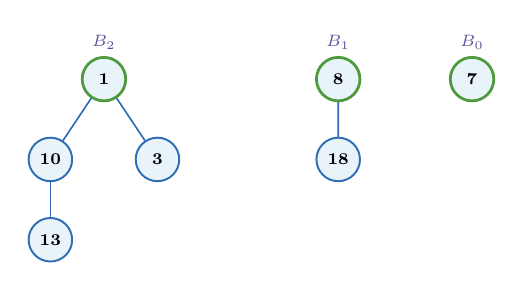
\begin{tikzpicture}[
  nd/.style={circle, draw=heapblue, line width=0.7pt, minimum size=6.5mm, inner sep=0pt, fill=skyfill, font=\scriptsize\bfseries},
  scale=0.85, transform shape
]
% B_2 (root 1)
\node[nd, draw=greenO, line width=1pt] (r1) at (0,0) {1};
\node[nd] (n10) at (-0.8,-1.2) {10};
\node[nd] (n3) at (0.8,-1.2) {3};
\node[nd] (n13) at (-0.8,-2.4) {13};
\draw[heapblue, line width=0.6pt] (r1)--(n10);
\draw[heapblue, line width=0.6pt] (r1)--(n3);
\draw[heapblue, line width=0.6pt] (n10)--(n13);
\node[font=\scriptsize\bfseries\color{violetT}] at (0,0.55) {$B_2$};

% B_1 (root 8)
\node[nd, draw=greenO, line width=1pt] (r8) at (3.5,0) {8};
\node[nd] (n18) at (3.5,-1.2) {18};
\draw[heapblue, line width=0.6pt] (r8)--(n18);
\node[font=\scriptsize\bfseries\color{violetT}] at (3.5,0.55) {$B_1$};

% B_0 (root 7)
\node[nd, draw=greenO, line width=1pt] (r7) at (5.5,0) {7};
\node[font=\scriptsize\bfseries\color{violetT}] at (5.5,0.55) {$B_0$};
\end{tikzpicture}
\end{center}

\textcolor{heapblue}{\textbf{Total key comparisons:}} $0+1+0+2+0+1+0 = 4 = n - \alpha(n) = 7 - 3$
\end{examplebox}

\begin{keybox}[Important Facts]
\renewcommand{\arraystretch}{1.4}
\begin{tabular}{l l}
Each edge & corresponds to exactly \textbf{one key comparison} \\
Building from $n$ elements & takes $\textcolor{violetT}{O(n)}$ key comparisons total \\
\end{tabular}
\end{keybox}

% ==================================================================
\section{Memory Representation}

\subsection{Three Pointers Per Node}

\begin{keybox}[Pointer Structure]
Each node stores \textbf{three pointers} plus two data fields:

\begin{center}
\renewcommand{\arraystretch}{1.4}
\begin{tabular}{l l l}
\hline
\textbf{Field} & \textbf{Points To} & \textbf{Color}\\
\hline
\textcolor{rustW}{\textbf{PARENT}} & Parent node & \textcolor{rustW}{Red}\\
\texttt{key} & Element's key & (data)\\
\texttt{degree} & Number of children & (data)\\
\textcolor{greenO}{\textbf{CHILD}} & Leftmost child & \textcolor{greenO}{Green}\\
\textcolor{heapblue}{\textbf{SIBLING}} & Right sibling & \textcolor{heapblue}{Blue}\\
\hline
\end{tabular}
\end{center}

We need the \textcolor{rustW}{PARENT} pointer for Decrease Key (covered later).
\end{keybox}

\subsection{Visual vs.\ Memory Representation}

\begin{warnbox}[Visual diagram $\ne$ memory pointers]
When we draw a binomial heap, the lines are \textbf{edges} (parent to child).

In memory, the actual \textbf{pointers} are:
\begin{itemize}[leftmargin=1.4em,itemsep=2pt]
  \item \textcolor{rustW}{\textbf{PARENT}}: child $\to$ its parent (upward)
  \item \textcolor{greenO}{\textbf{LEFT CHILD}}: parent $\to$ its \textbf{leftmost} child only
  \item \textcolor{heapblue}{\textbf{RIGHT SIBLING}}: one child $\to$ the next sibling (across)
\end{itemize}
The visual edges are NOT pointers. Each visual edge is implemented through a combination of LEFT CHILD and RIGHT SIBLING pointers.
\end{warnbox}

\subsection{HEAD Pointer and Root List}

The roots of the $B_k$ trees are connected via \textcolor{heapblue}{\textbf{RIGHT SIBLING}} pointers, forming a \textbf{linked list of roots}. A \textbf{HEAD} pointer points to the root of the \textbf{smallest} tree (smallest $k$).

\begin{examplebox}[Memory Layout Example]
Heap: $\langle B_3(\text{root } 8),\; B_2(\text{root } 1),\; B_0(\text{root } 7) \rangle$

Root linked list:

\begin{center}
\texttt{HEAD} $\;\to\;$ \fbox{7} $\;\xrightarrow{\textcolor{heapblue}{\text{sib}}}\;$ \fbox{1} $\;\xrightarrow{\textcolor{heapblue}{\text{sib}}}\;$ \fbox{8} $\;\to\;$ \texttt{NIL}
\end{center}

HEAD points to 7 ($B_0$, smallest tree). Then 7's sibling pointer goes to 1 ($B_2$), then to 8 ($B_3$).

Here is a full pointer diagram for a smaller heap $\langle B_2(\text{root } 3),\; B_1(\text{root } 5),\; B_0(\text{root } 9) \rangle$:

\begin{center}
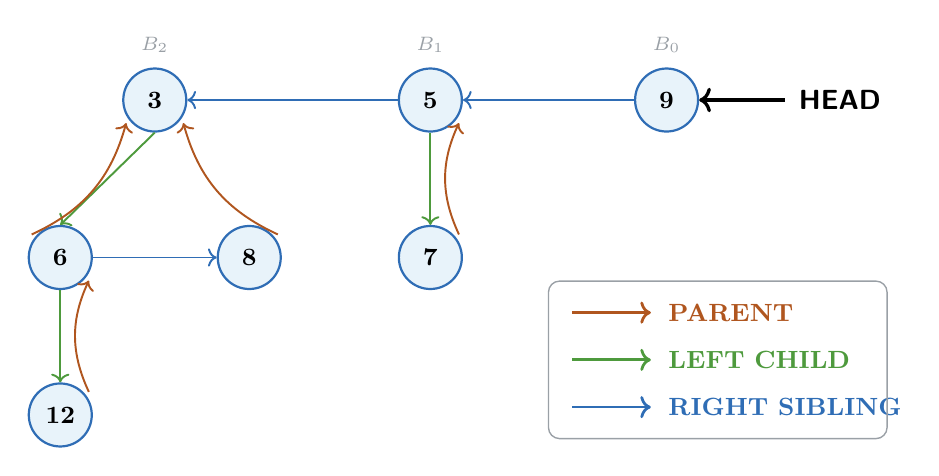
\begin{tikzpicture}[
  nd/.style={circle, draw=heapblue, line width=0.8pt, minimum size=8mm, inner sep=0pt, fill=skyfill, font=\small\bfseries},
]
% Root list (top row)
\node[nd] (n9) at (8,0) {9};
\node[nd] (n5) at (5,0) {5};
\node[nd] (n3) at (1.5,0) {3};

% HEAD
\node[font=\bfseries] at (10.2,0) {\textsf{HEAD}};
\draw[->, line width=1.2pt] (9.5,0) -- (n9);

% Root sibling pointers (blue, right to left)
\draw[->, heapblue, line width=0.7pt] (n9.west) -- (n5.east);
\draw[->, heapblue, line width=0.7pt] (n5.west) -- (n3.east);

% Tree labels above
\node[font=\scriptsize\color{greyline}] at (8,0.7) {$B_0$};
\node[font=\scriptsize\color{greyline}] at (5,0.7) {$B_1$};
\node[font=\scriptsize\color{greyline}] at (1.5,0.7) {$B_2$};

% Under 5 (B_1): left child = 7
\node[nd] (n7) at (5,-2) {7};
\draw[->, greenO, line width=0.7pt] (n5.south) -- (n7.north);
\draw[->, rustW, line width=0.7pt] ([xshift=2pt]n7.north east) to[bend left=25] ([xshift=2pt]n5.south east);

% Under 3 (B_2): left child = 6, sibling = 8
\node[nd] (n6) at (0.3,-2) {6};
\node[nd] (n8) at (2.7,-2) {8};
\draw[->, greenO, line width=0.7pt] (n3.south) -- (n6.north);
\draw[->, heapblue, line width=0.7pt] (n6.east) -- (n8.west);
\draw[->, rustW, line width=0.7pt] ([xshift=-2pt]n6.north west) to[bend right=25] ([xshift=-2pt]n3.south west);
\draw[->, rustW, line width=0.7pt] ([xshift=2pt]n8.north east) to[bend left=25] ([xshift=2pt]n3.south east);

% Under 6: left child = 12
\node[nd] (n12) at (0.3,-4) {12};
\draw[->, greenO, line width=0.7pt] (n6.south) -- (n12.north);
\draw[->, rustW, line width=0.7pt] ([xshift=2pt]n12.north east) to[bend left=25] ([xshift=2pt]n6.south east);

% Legend
\draw[->, rustW, line width=1pt] (6.8,-2.7) -- (7.8,-2.7);
\node[font=\small\bfseries, anchor=west, text=rustW] at (7.9,-2.7) {PARENT};
\draw[->, greenO, line width=1pt] (6.8,-3.3) -- (7.8,-3.3);
\node[font=\small\bfseries, anchor=west, text=greenO] at (7.9,-3.3) {LEFT CHILD};
\draw[->, heapblue, line width=1pt] (6.8,-3.9) -- (7.8,-3.9);
\node[font=\small\bfseries, anchor=west, text=heapblue] at (7.9,-3.9) {RIGHT SIBLING};
\draw[rounded corners, greyline, line width=0.5pt] (6.5,-2.3) rectangle (10.8,-4.3);
\end{tikzpicture}
\end{center}
\end{examplebox}

% ==================================================================
\section{Two Key Lemmas}

Before the operations, we need two building blocks. These lemmas are \textbf{the reason} all operations work efficiently.

\subsection{Lemma 1: Merging Two $B_k$ Trees}

\begin{keybox}[Lemma 1]
We can merge \textcolor{rustW}{two} min heap ordered $B_k$ trees into a \textcolor{greenO}{single} min heap ordered $B_{k+1}$ tree using just \textcolor{violetT}{\textbf{one}} key comparison.
\end{keybox}

\begin{keybox}[Why Lemma 1 Matters]
This is the \textbf{carry operation}. Just like adding two 1 bits produces a carry in binary addition, merging two $B_k$'s produces one $B_{k+1}$. This is the core mechanism behind Union, Insert, and Extract\_Min.
\end{keybox}

\textbf{Proof.} Given two $B_k$ trees with roots $x$ and $y$:

\begin{enumerate}[leftmargin=1.4em,itemsep=3pt]
  \item Compare $x.\text{key}$ and $y.\text{key}$ \quad (one comparison).
  \item Smaller root stays on top. Make the other tree the new leftmost subtree.
\end{enumerate}

If $x \le y$: $x$ is root of $B_{k+1}$, with children $B_k(y),\, B_{k-1},\, \ldots,\, B_0$.

Min heap ordering preserved (smaller root on top). Structure is $B_{k+1}$ by definition. \hfill $\square$

\begin{examplebox}[Lemma 1 in Action: Merging Two $B_1$'s into $B_2$]
Two min heap ordered $B_1$ trees. One comparison decides the root.

\begin{center}
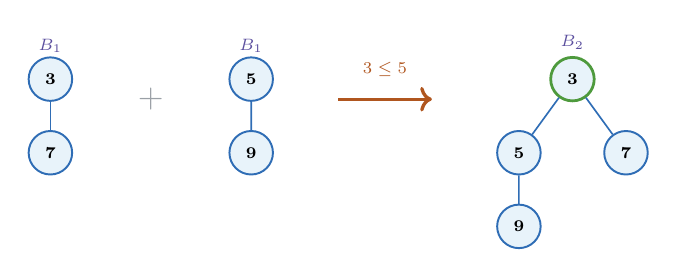
\begin{tikzpicture}[
  nd/.style={circle, draw=heapblue, line width=0.7pt, minimum size=6.5mm, inner sep=0pt, fill=skyfill, font=\scriptsize\bfseries},
  scale=0.85, transform shape
]
% Left B_1
\node[nd] (a) at (0,0) {3};
\node[nd] (a1) at (0,-1.1) {7};
\draw[heapblue, line width=0.6pt] (a)--(a1);
\node[font=\scriptsize\bfseries\color{violetT}] at (0,0.5) {$B_1$};

% Plus
\node[font=\Large\bfseries\color{greyline}] at (1.5,-0.3) {$+$};

% Right B_1
\node[nd] (b) at (3,0) {5};
\node[nd] (b1) at (3,-1.1) {9};
\draw[heapblue, line width=0.6pt] (b)--(b1);
\node[font=\scriptsize\bfseries\color{violetT}] at (3,0.5) {$B_1$};

% Arrow
\draw[->, line width=1.2pt, rustW] (4.3,-0.3) -- (5.7,-0.3);
\node[font=\scriptsize\bfseries\color{rustW}] at (5,0.15) {$3 \le 5$};

% Result B_2
\node[nd, draw=greenO, line width=1pt] (r) at (7.8,0) {3};
\node[nd] (r1) at (7,-1.1) {5};
\node[nd] (r2) at (8.6,-1.1) {7};
\node[nd] (r3) at (7,-2.2) {9};
\draw[heapblue, line width=0.6pt] (r)--(r1);
\draw[heapblue, line width=0.6pt] (r)--(r2);
\draw[heapblue, line width=0.6pt] (r1)--(r3);
\node[font=\scriptsize\bfseries\color{violetT}] at (7.8,0.55) {$B_2$};
\end{tikzpicture}
\end{center}

$3 \le 5$, so 3 stays as root. The other tree (root 5) becomes the \textbf{new leftmost child}. One comparison, one new edge.
\end{examplebox}

\subsection{Lemma 2: Deleting the Root of $B_k$}

\begin{keybox}[Lemma 2]
Deleting \textcolor{rustW}{the root} of a min heap ordered $B_k$ gives a valid \textcolor{greenO}{min binomial heap} of $2^k - 1$ elements.
\end{keybox}

\begin{keybox}[Why Lemma 2 Matters]
This is the key insight behind Extract\_Min. When we extract the minimum (a root of some $B_k$ tree), the remaining children form their own binomial heap. We then Union that new heap back with the rest.
\end{keybox}

\textbf{Proof.} Root of $B_k$ has children $B_{k-1}, B_{k-2}, \ldots, B_1, B_0$.

Delete the root $\Rightarrow$ left with these $k$ subtrees. Each is already min heap ordered (removing the root does not affect subtrees). The sequence $\langle B_{k-1}, \ldots, B_1, B_0 \rangle$ is a valid binomial forest (strictly decreasing $k$ values), so it is a binomial heap of size $2^{k-1} + \cdots + 1 = 2^k - 1$. \hfill $\square$

% ==================================================================
\section{Operations}

\begin{keybox}[The Big Picture]
\textbf{Everything reduces to Union.}
\begin{itemize}[leftmargin=1.4em,itemsep=2pt]
  \item Insert = Union with a tiny heap (single $B_0$)
  \item Extract\_Min = remove a root (Lemma 2 gives a new heap) + Union
  \item Union itself = binary addition using Lemma 1 as the carry
\end{itemize}
Lemma 1 ($O(1)$ merge) and Lemma 2 (delete root $\Rightarrow$ valid heap) are the two pillars.
\end{keybox}

\subsection{Union($T$, $Q$): Merging Two Binomial Heaps}

\begin{defbox}[Union($T$, $Q$)]
\textbf{Input:} two min binomial heaps $T$ and $Q$.\\
\textbf{Output:} a single min binomial heap $S$ containing all elements.

\textbf{Algorithm:} Binary addition!

Each column (bit position $i$) can have 0, 1, 2, or 3 copies of $B_i$ (from $T$, from $Q$, plus possibly a carry from position $i-1$). Process right to left:
\begin{itemize}[leftmargin=1.4em,itemsep=2pt]
  \item \textbf{0 trees}: nothing in $S$, no carry
  \item \textbf{1 tree}: put it in $S$, no carry
  \item \textbf{2 trees}: merge via Lemma 1 into $B_{i+1}$, carry it. Nothing in $S$ at position $i$.
  \item \textbf{3 trees}: put one in $S$, merge the other two into a carry
\end{itemize}
\end{defbox}

\begin{examplebox}[Full Worked Example: Union($T$, $Q$)]
$T$ has size $3 = \langle 11 \rangle_2$, so $T = \langle B_1, B_0 \rangle$.\\
$Q$ has size $7 = \langle 111 \rangle_2$, so $Q = \langle B_2, B_1, B_0 \rangle$.

Result: $3 + 7 = 10 = \langle 1010 \rangle_2$, so $S = \langle B_3, B_1 \rangle$.

\textbf{Concrete values:}
\begin{itemize}[leftmargin=1.4em,itemsep=1pt]
  \item $T$: $B_1$(root 2, child 4). $B_0$(root 3).
  \item $Q$: $B_2$(root 5, children: 7$\to$9 and 10). $B_1$(root 1, child 8). $B_0$(root 6).
\end{itemize}

\begin{center}
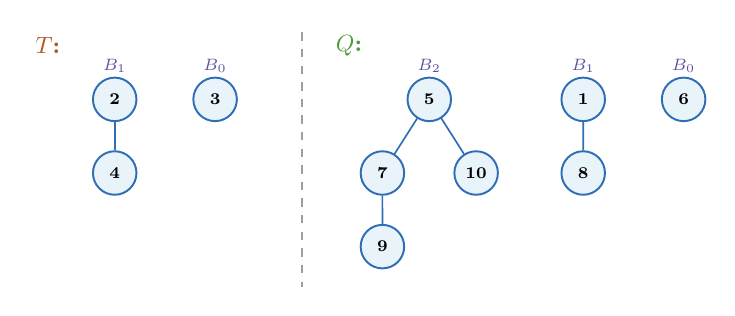
\begin{tikzpicture}[
  nd/.style={circle, draw=heapblue, line width=0.7pt, minimum size=6.5mm, inner sep=0pt, fill=skyfill, font=\scriptsize\bfseries},
  scale=0.85, transform shape
]
% T
\node[font=\bfseries\color{rustW}] at (-0.5,0.8) {$T$:};
\node[nd] (t2) at (0.5,0) {2};
\node[nd] (t4) at (0.5,-1.1) {4};
\draw[heapblue, line width=0.6pt] (t2)--(t4);
\node[font=\scriptsize\color{violetT}] at (0.5,0.5) {$B_1$};
\node[nd] (t3) at (2,0) {3};
\node[font=\scriptsize\color{violetT}] at (2,0.5) {$B_0$};
% divider
\draw[greyline, dashed, line width=0.5pt] (3.3,1) -- (3.3,-2.8);
% Q
\node[font=\bfseries\color{greenO}] at (4,0.8) {$Q$:};
\node[nd] (q5) at (5.2,0) {5};
\node[nd] (q7) at (4.5,-1.1) {7};
\node[nd] (q10) at (5.9,-1.1) {10};
\node[nd] (q9) at (4.5,-2.2) {9};
\draw[heapblue, line width=0.6pt] (q5)--(q7); \draw[heapblue, line width=0.6pt] (q5)--(q10);
\draw[heapblue, line width=0.6pt] (q7)--(q9);
\node[font=\scriptsize\color{violetT}] at (5.2,0.5) {$B_2$};
\node[nd] (q1) at (7.5,0) {1};
\node[nd] (q8) at (7.5,-1.1) {8};
\draw[heapblue, line width=0.6pt] (q1)--(q8);
\node[font=\scriptsize\color{violetT}] at (7.5,0.5) {$B_1$};
\node[nd] (q6) at (9,0) {6};
\node[font=\scriptsize\color{violetT}] at (9,0.5) {$B_0$};
\end{tikzpicture}
\end{center}

\textbf{\textcolor{violetT}{Position 0} ($B_0$ column):}

$T$ has $B_0$(3), $Q$ has $B_0$(6). Two trees $\Rightarrow$ merge.

Compare 3 vs 6: $3 \le 6 \Rightarrow B_1$(root 3, child 6). This is the \textbf{carry}.

$S$ at position 0: empty.\\[6pt]

\textbf{\textcolor{violetT}{Position 1} ($B_1$ column):}

$T$ has $B_1$(root 2), $Q$ has $B_1$(root 1), plus carry $B_1$(root 3). \textcolor{rustW}{Three trees!}

Keep one in $S$: the carry $B_1$(3$\to$6).

Merge the other two: compare 1 vs 2: $1 \le 2 \Rightarrow B_2$(root 1, with subtrees from both). New carry.

$S$ at position 1: $B_1$(root 3, child 6).\\[6pt]

\textbf{\textcolor{violetT}{Position 2} ($B_2$ column):}

$Q$ has $B_2$(root 5), plus carry $B_2$(root 1). Two trees $\Rightarrow$ merge.

Compare 1 vs 5: $1 \le 5 \Rightarrow B_3$(root 1). Carry to position 3.

$S$ at position 2: empty.\\[6pt]

\textbf{\textcolor{violetT}{Position 3} ($B_3$ column):}

Just the carry $B_3$(root 1). One tree $\Rightarrow$ done.

$S$ at position 3: $B_3$(root 1).\\[6pt]

\textbf{\textcolor{violetT}{Result:}} $S = \langle B_3(\text{root } 1),\; B_1(\text{root } 3) \rangle$ \qquad $10 = \langle 1010 \rangle_2$ \checkmark

\begin{center}
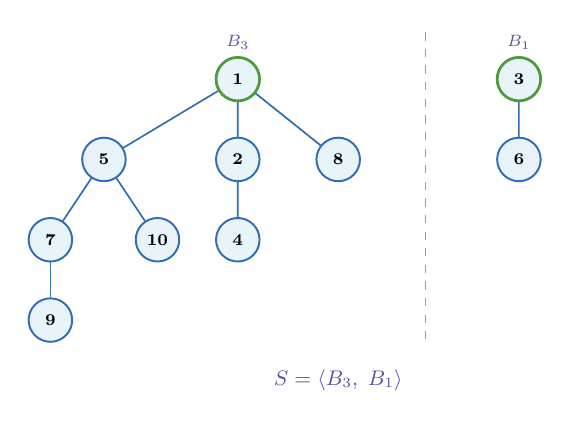
\begin{tikzpicture}[
  nd/.style={circle, draw=heapblue, line width=0.7pt, minimum size=6.5mm, inner sep=0pt, fill=skyfill, font=\scriptsize\bfseries},
  scale=0.85, transform shape
]
% B_3 (root 1)
\node[nd, draw=greenO, line width=1pt] (r1) at (2,0) {1};
\node[font=\scriptsize\bfseries\color{violetT}] at (2,0.55) {$B_3$};
% Children: B_2(5), B_1(2), B_0(8)
\node[nd] (n5) at (0,-1.2) {5};
\node[nd] (n2) at (2,-1.2) {2};
\node[nd] (n8) at (3.5,-1.2) {8};
\draw[heapblue, line width=0.6pt] (r1)--(n5);
\draw[heapblue, line width=0.6pt] (r1)--(n2);
\draw[heapblue, line width=0.6pt] (r1)--(n8);
% Children of 5: B_1(7), B_0(10)
\node[nd] (n7) at (-0.8,-2.4) {7};
\node[nd] (n10) at (0.8,-2.4) {10};
\draw[heapblue, line width=0.6pt] (n5)--(n7);
\draw[heapblue, line width=0.6pt] (n5)--(n10);
% Child of 7: B_0(9)
\node[nd] (n9) at (-0.8,-3.6) {9};
\draw[heapblue, line width=0.6pt] (n7)--(n9);
% Child of 2: B_0(4)
\node[nd] (n4) at (2,-2.4) {4};
\draw[heapblue, line width=0.6pt] (n2)--(n4);

% Separator
\draw[greyline, dashed, line width=0.5pt] (4.8,0.7) -- (4.8,-4);

% B_1 (root 3)
\node[nd, draw=greenO, line width=1pt] (r3) at (6.2,0) {3};
\node[font=\scriptsize\bfseries\color{violetT}] at (6.2,0.55) {$B_1$};
\node[nd] (n6) at (6.2,-1.2) {6};
\draw[heapblue, line width=0.6pt] (r3)--(n6);

% Label
\node[font=\small\bfseries\color{violetT}] at (3.5,-4.5) {$S = \langle B_3,\; B_1 \rangle$};
\end{tikzpicture}
\end{center}

\textbf{\textcolor{heapblue}{New edges:}} 3 \qquad \textbf{\textcolor{heapblue}{Key comparisons:}} 3
\end{examplebox}

\begin{keybox}[Union Complexity]
If $|T| \le n$ and $|Q| \le n$, each heap has $\le \lfloor \log_2 n \rfloor + 1$ trees.

$\Rightarrow$ Union takes $\textcolor{violetT}{O(\log n)}$ comparisons (one per column of the binary addition).
\end{keybox}

\subsection{Insert($T$, $x$): Adding a Single Element}

\begin{defbox}[Insert($T$, $x$)]
\begin{enumerate}[leftmargin=1.4em,itemsep=2pt]
  \item Create a new heap $Q$ containing just $x$ (a single $B_0$).
  \item Return Union($T$, $Q$).
\end{enumerate}
\end{defbox}

\begin{keybox}[Insert = Adding 1 in Binary]
If the last bit is 0 (no $B_0$ exists): place the new $B_0$. Done in $O(1)$.

If the last bit is 1: merge into $B_1$ (carry). If $B_1$ already exists, merge again into $B_2$. This cascading carry can go up to $O(\log n)$ positions, but on average much less.
\end{keybox}

\begin{examplebox}[Insert Example]
Heap $T = \langle B_2, B_0 \rangle$ (5 elements, binary $101$). Insert element $x$.

\begin{enumerate}[leftmargin=1.4em,itemsep=2pt]
  \item $x$ becomes $B_0$. Now two $B_0$'s.
  \item Merge them $\Rightarrow$ one $B_1$ (carry). No $B_1$ exists, so $B_1$ stays.
  \item Result: $\langle B_2, B_1 \rangle$ (6 elements, binary $110$). \checkmark
\end{enumerate}
\end{examplebox}

\subsection{Min($T$): Finding the Minimum}

\begin{defbox}[Min($T$)]
The minimum element is the root of one of the trees (by min heap property).

Walk through the root list (linked list via HEAD pointer). Compare each root's key. Return the smallest.

At most $\lfloor \log_2 n \rfloor + 1$ roots $\Rightarrow$ $\textcolor{violetT}{O(\log n)}$.
\end{defbox}

\subsection{Extract\_Min($T$): Remove the Minimum}

\begin{defbox}[Extract\_Min($T$)]
\begin{enumerate}[leftmargin=1.4em,itemsep=3pt]
  \item \textbf{Find the min:} walk the root list to find the tree $B_k$ whose root has the smallest key. \hfill $O(\log n)$
  \item \textbf{Remove that tree} from the heap $T$. \hfill $O(1)$
  \item \textbf{Delete the root} of $B_k$. By \textbf{Lemma 2}, the children form a new binomial heap $Q = \langle B_{k-1}, \ldots, B_0 \rangle$. \hfill $O(\log n)$
  \item \textbf{Union}$(T, Q)$. \hfill $O(\log n)$
\end{enumerate}
Total: $\textcolor{violetT}{O(\log n)}$.
\end{defbox}

\begin{examplebox}[Extract\_Min Example]
Heap: $\langle B_3(\text{root } 1),\; B_1(\text{root } 3) \rangle$ (10 elements)

\begin{enumerate}[leftmargin=1.4em,itemsep=2pt]
  \item Min = 1 (root of $B_3$).
  \item Remove $B_3$ from heap. Remaining: $\langle B_1(\text{root } 3) \rangle$.
  \item Delete root 1 from $B_3$. Children: $B_2, B_1, B_0$. New heap $Q = \langle B_2, B_1, B_0 \rangle$ (7 elements).
  \item Union($\langle B_1 \rangle$, $\langle B_2, B_1, B_0 \rangle$):

  Position 0: one $B_0$ $\Rightarrow$ stays.

  Position 1: two $B_1$'s $\Rightarrow$ merge into $B_2$ (carry).

  Position 2: two $B_2$'s $\Rightarrow$ merge into $B_3$ (carry).

  Position 3: one $B_3$ $\Rightarrow$ stays.

  Result: $\langle B_3, B_0 \rangle$ (9 elements, $9 = \langle 1001 \rangle_2$) \checkmark
\end{enumerate}

Return 1.
\end{examplebox}

% ==================================================================
\section{Complexity Summary}

\begin{keybox}[Binomial Heap Operations]
\renewcommand{\arraystretch}{1.5}
\begin{tabular}{l c l}
\textbf{\textcolor{violetT}{Operation}} & \textbf{Worst Case} & \textbf{Key Insight}\\
\hline
\texttt{Union($T$, $Q$)} & $\textcolor{violetT}{O(\log n)}$ & binary addition \\
\texttt{Insert($T$, $x$)} & $\textcolor{violetT}{O(\log n)}$ & Union with single $B_0$ \\
\texttt{Min($T$)} & $\textcolor{violetT}{O(\log n)}$ & scan root list \\
\texttt{Extract\_Min($T$)} & $\textcolor{violetT}{O(\log n)}$ & Lemma 2 + Union \\
\end{tabular}
\end{keybox}

% ==================================================================
\section{Practice Problems}

\begin{examplebox}[Problem 1: Build a Binomial Heap]
Build a min binomial heap by inserting: $5, 12, 3, 9, 2, 15, 6, 1$.

(a) How many trees does the final heap have?\\
(b) What is the root of each tree?\\
(c) How many total key comparisons?

\begin{answerband}
$n = 8 = \langle 1000 \rangle_2 \Rightarrow F_8 = \langle B_3 \rangle$ (one tree).

Step by step:
\begin{itemize}[leftmargin=1.4em,itemsep=1pt]
  \item Insert 5: $\langle B_0(5) \rangle$. \hfill 0 comps
  \item Insert 12: merge $B_0$'s: $5 \le 12$. $\langle B_1(5 \to 12) \rangle$. \hfill 1 comp
  \item Insert 3: $\langle B_1(5), B_0(3) \rangle$. \hfill 0 comps
  \item Insert 9: merge $B_0$'s: $3 \le 9$. Two $B_1$'s: $3 \le 5$. $\langle B_2(\text{root } 3) \rangle$. \hfill 2 comps
  \item Insert 2: $\langle B_2(3), B_0(2) \rangle$. \hfill 0 comps
  \item Insert 15: merge $B_0$'s: $2 \le 15$. $\langle B_2(3), B_1(2 \to 15) \rangle$. \hfill 1 comp
  \item Insert 6: $\langle B_2(3), B_1(2), B_0(6) \rangle$. \hfill 0 comps
  \item Insert 1: merge $B_0$'s: $1 \le 6$. Two $B_1$'s: $1 \le 2$. Two $B_2$'s: $1 \le 3$. $\langle B_3(\text{root } 1) \rangle$. \hfill 3 comps
\end{itemize}

(a) \textcolor{violetT}{1 tree.} \quad (b) \textcolor{violetT}{Root is 1.} \quad (c) \textcolor{violetT}{$1+0+2+0+1+0+3 = 7 = n - \alpha(n) = 8 - 1$}
\end{answerband}
\end{examplebox}

\begin{examplebox}[Problem 2: Extract\_Min]
Given: $\langle B_2(\text{root } 3, \text{children: } 7 \to 9 \text{ and } 5),\; B_0(\text{root } 10) \rangle$. Perform Extract\_Min.

\begin{answerband}
\begin{enumerate}[leftmargin=1.4em,itemsep=2pt]
  \item Min = 3 (root of $B_2$). Extract it.
  \item Remove $B_2$. Remaining: $\langle B_0(10) \rangle$.
  \item Root 3 had children: $B_1$(root 7, child 9) and $B_0$(root 5). New heap $Q = \langle B_1(7 \to 9), B_0(5) \rangle$.
  \item Union($\langle B_0(10) \rangle$, $\langle B_1(7), B_0(5) \rangle$):

  Position 0: two $B_0$'s (10, 5). $5 \le 10 \Rightarrow B_1$(root 5, child 10). Carry.

  Position 1: $B_1$(root 7) + carry $B_1$(root 5). $5 \le 7 \Rightarrow B_2$(root 5). Carry.

  Position 2: just carry. Done.

  Result: $\langle B_2(\text{root } 5) \rangle$ (4 elements, $4 = \langle 100 \rangle_2$) \checkmark
\end{enumerate}

Return 3.
\end{answerband}
\end{examplebox}

\begin{examplebox}[Problem 3: Properties Quick Check]
For $B_5$:

\begin{center}
\renewcommand{\arraystretch}{1.3}
\begin{tabular}{l l}
Nodes? & \textcolor{violetT}{$2^5 = 32$} \\
Height? & \textcolor{violetT}{$5$} \\
Degree of root? & \textcolor{violetT}{$5$} \\
Nodes at depth 2? & \textcolor{violetT}{$\binom{5}{2} = 10$} \\
Nodes at depth 5? & \textcolor{violetT}{$\binom{5}{5} = 1$} \\
\end{tabular}
\end{center}

For $F_{13}$ ($13 = \langle 1101 \rangle_2$):

\begin{center}
\renewcommand{\arraystretch}{1.3}
\begin{tabular}{l l}
Which trees? & \textcolor{violetT}{$\langle B_3, B_2, B_0 \rangle$} \\
How many trees? & \textcolor{violetT}{$\alpha(13) = 3$} \\
How many edges? & \textcolor{violetT}{$13 - 3 = 10$} \\
\end{tabular}
\end{center}
\end{examplebox}

% ==================================================================
\section{Exam Relevance}

Based on past CSC263 exams (2012 through 2015), no specific binomial heap questions appeared. However, heap questions show up frequently. The $k$Set ADT problem from Fall 2014 (see Lecture 2 notes) used max heaps and min heaps together.

\begin{warnbox}[What to watch for on binomial heap questions]
\begin{itemize}[leftmargin=1.4em,itemsep=2pt]
  \item ``Draw the binomial heap after inserting $x_1, x_2, \ldots$'' $\Rightarrow$ binary addition method
  \item ``Show the result of Extract\_Min'' $\Rightarrow$ Lemma 2 + Union
  \item ``How many key comparisons?'' $\Rightarrow$ count new edges = count merges
  \item ``Why $O(\log n)$?'' $\Rightarrow$ at most $\lfloor \log_2 n \rfloor + 1$ trees, binary addition has that many columns
\end{itemize}
\end{warnbox}

% ==================================================================
\section*{\textcolor{violetT}{Quick Reference: Lecture 3}}
\addcontentsline{toc}{section}{Quick Reference: Lecture 3}
\begin{keybox}
\renewcommand{\arraystretch}{1.4}
\begin{tabular}{l l}
$B_k$ & two $B_{k-1}$'s merged; has $2^k$ nodes, height $k$, $\binom{k}{d}$ at depth $d$\\
$F_n$ & forest of $B_k$'s matching 1 bits of $n$; has $\alpha(n)$ trees, $n{-}\alpha(n)$ edges\\
Min Binomial Heap & $F_n$ + one element per node + min heap ordering\\
Memory & 3 pointers: \textcolor{rustW}{PARENT}, \textcolor{greenO}{LEFT CHILD}, \textcolor{heapblue}{RIGHT SIBLING}; HEAD $\to$ root list\\
Lemma 1 & merge two $B_k \to B_{k+1}$ with 1 comparison (the ``carry'')\\
Lemma 2 & delete root of $B_k \to$ valid heap of $2^k{-}1$ elements\\
\textbf{Union} & binary addition $\to$ $O(\log n)$\\
\textbf{Insert} & Union with $B_0$ $\to$ $O(\log n)$\\
\textbf{Min} & scan root list $\to$ $O(\log n)$\\
\textbf{Extract\_Min} & Lemma 2 + Union $\to$ $O(\log n)$\\
\end{tabular}
\end{keybox}


% ******************************************************************
%  LECTURE 4 — IMPROVED VERSION
%
%  PASTE INSTRUCTIONS:
%  1. In your master document, find the line:
%       \part*{\textcolor{utnavy}{Lecture 4: Binomial Heaps (Part 2) + Binary Search Trees}}
%  2. DELETE everything from that line down to (and including):
%       \end{document}
%  3. Paste EVERYTHING below in its place.
% ******************************************************************

\part*{\textcolor{utnavy}{Lecture 4: Binomial Heaps (Part 2) + Binary Search Trees}}
\addcontentsline{toc}{part}{Lecture 4: Binomial Heaps (Part 2) + BST}

% ==================================================================
\section{Remaining Binomial Heap Operations}

Recall from Lecture 3: a \textcolor{rustW}{Min Binomial Heap} $T$ is a forest of binomial trees $B_{k_1}, B_{k_2}, \ldots$, each satisfying the \textcolor{rustW}{min-heap property} (parent key $\leq$ children keys). Every node stores three pointers: \textcolor{rustW}{PARENT}, \textcolor{greenO}{LEFT CHILD}, \textcolor{heapblue}{RIGHT SIBLING}.

We already have Union, Insert, Min, Extract\_Min — all $O(\log n)$. Now we add three more operations that \textbf{modify a specific node} we already have a pointer to.

\subsection{Decrease\_Key$(T, x, k)$: Make a Key Smaller}

\textcolor{heapblue}{\textbf{Goal:}} change the key of node $x$ to a \textbf{smaller} value $k$ (where $k < x.\text{key}$).

\textbf{Why would we want this?} Shortest-path algorithms (Dijkstra's) update distances as they find shorter paths. A priority queue needs to let you say ``this element is now more urgent.''

\begin{defbox}[Decrease\_Key$(T, x, k)$]
\textbf{Precondition:} we have a \textbf{direct pointer} to node $x$. No searching needed.

\textbf{Algorithm:}
\begin{enumerate}[leftmargin=1.4em,itemsep=2pt]
    \item Set $x.\text{key} \leftarrow k$
    \item \textcolor{rustW}{Bubble up}: while $x$ is not a root \textbf{and} $x.\text{key} < x.\text{parent}.\text{key}$:
    \begin{itemize}[leftmargin=1.2em]
        \item swap $x.\text{key}$ with $x.\text{parent}.\text{key}$
        \item move $x$ pointer up to the parent
    \end{itemize}
    \item Stop when min-heap property is restored (parent's key $\leq x.\text{key}$) or $x$ is a root
\end{enumerate}
\end{defbox}

\begin{keybox}[Why ``Bubble Up'' Works]
We decreased $x$'s key, so the only possible violation is $x.\text{key} < x.\text{parent}.\text{key}$ (child smaller than parent). Swapping with parent fixes this violation but might create a new one further up. We keep going until we reach a parent whose key is $\leq$ ours, or we hit the root.

The \textcolor{rustW}{PARENT pointer} (from Lecture 3's memory representation) is what makes this efficient — we can walk straight up without searching.
\end{keybox}

\textbf{Complexity:} \textcolor{greenO}{$O(\log n)$}

At most we bubble up from the deepest node to the root. In a binomial tree $B_k$, the height is $k$. The largest tree in a heap of $n$ elements is at most $B_{\lfloor \log_2 n \rfloor}$, so we do at most $\lfloor \log_2 n \rfloor$ swaps.

\begin{examplebox}[Worked Example: Decrease\_Key]
Suppose we have $B_3$ (8 nodes, height 3) with keys arranged as:

\begin{center}
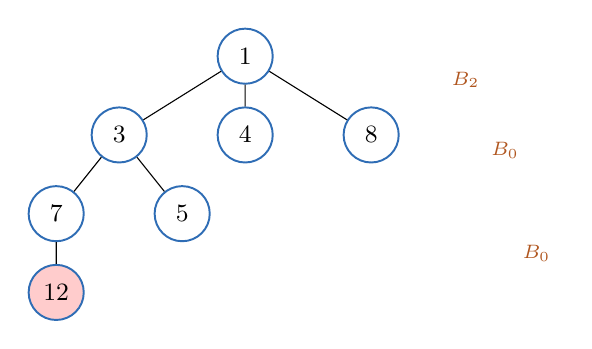
\begin{tikzpicture}[
    level distance=1cm, sibling distance=1.6cm,
    every node/.style={circle, draw=heapblue, line width=0.7pt, minimum size=7mm, inner sep=1pt, font=\small, fill=white}
]
\node {1}
    child {node {3}
        child {node {7}
            child {node[fill=red!20] (target) {12}}
        }
        child {node {5}}
    }
    child {node {4}}
    child {node {8}};
\node[draw=none, fill=none, font=\scriptsize\itshape, text=rustW] at (2.8, -0.3) {$B_2$};
\node[draw=none, fill=none, font=\scriptsize\itshape, text=rustW] at (3.3, -1.2) {$B_0$};
\node[draw=none, fill=none, font=\scriptsize\itshape, text=rustW] at (3.7, -2.5) {$B_0$};
\end{tikzpicture}
\end{center}

\texttt{Decrease\_Key$(T, x, 2)$} where $x$ is the node with key 12:

\begin{enumerate}[leftmargin=1.4em,itemsep=2pt]
    \item Set $x.\text{key} = 2$
    \item Compare with parent (key 7): $2 < 7$ $\Rightarrow$ swap. Now 2 is at depth 2, 7 is at depth 3.
    \item Compare with parent (key 3): $2 < 3$ $\Rightarrow$ swap. Now 2 is at depth 1, 3 is at depth 2.
    \item Compare with parent (key 1): $2 > 1$ $\Rightarrow$ \textcolor{greenO}{STOP}. Min-heap property restored.
\end{enumerate}

Total swaps: 2 (out of max 3 = height of $B_3$). The tree is still a valid $B_3$ with min-heap ordering.
\end{examplebox}

\subsection{Delete$(T, x)$: Remove a Specific Node}

\textcolor{heapblue}{\textbf{Goal:}} remove node $x$ from $T$. Again, we have a direct pointer to $x$.

\textbf{The trick:} we already know how to remove a \textit{root} (Extract\_Min). So force $x$ to become a root first!

\begin{defbox}[Delete$(T, x)$]
\begin{enumerate}[leftmargin=1.4em,itemsep=3pt]
    \item \texttt{Decrease\_Key$(T, x, -\infty)$}: set $x$'s key to $-\infty$. Since $-\infty$ is smaller than every other key, $x$ bubbles \textbf{all the way up} to become the root of its binomial tree.
    \item \texttt{Extract\_Min$(T)$}: the minimum element is now $x$ (with key $-\infty$), so Extract\_Min removes it. Internally this uses Lemma 2 (children of $x$'s tree form a new heap) + Union.
\end{enumerate}
\end{defbox}

\textbf{Complexity:} \textcolor{greenO}{$O(\log n)$} \quad (Decrease\_Key $O(\log n)$ + Extract\_Min $O(\log n)$)

\subsection{Increase\_Key$(T, x, k)$: Make a Key Larger}

\textcolor{heapblue}{\textbf{Goal:}} change the key of node $x$ to a \textbf{larger} value $k$ (where $k > x.\text{key}$).

\begin{warnbox}[Why can't we just ``bubble down''?]
When we \textit{decrease} a key, the only violation is with the parent (one node above), and we bubble up along a single path.

When we \textit{increase} a key, the violation is with the \textbf{children}. In a binomial tree, a node in $B_k$ can have up to $k$ children. To bubble down:
\begin{enumerate}[leftmargin=1.4em,itemsep=1pt]
    \item We need to find the \textbf{minimum-key child} among all children (to maintain min-heap property after swap).
    \item A node in $B_k$ can have up to $k$ children $\Rightarrow$ scanning children costs $O(k)$ per level.
    \item There are up to $k$ levels to descend.
    \item Total: $O(k^2) = O(\log^2 n)$. That is \textbf{worse} than $O(\log n)$!
\end{enumerate}
\end{warnbox}

\textbf{Better approach — Delete + re-Insert:}

\begin{defbox}[Increase\_Key$(T, x, k)$]
\begin{enumerate}[leftmargin=1.4em,itemsep=2pt]
    \item \texttt{Delete$(T, x)$}: remove $x$ entirely. \hfill $O(\log n)$
    \item Create a new node $x'$ with key $k$.
    \item \texttt{Insert$(T, x')$}: add $x'$ back via Union. \hfill $O(\log n)$
\end{enumerate}
\end{defbox}

\textbf{Complexity:} \textcolor{greenO}{$O(\log n)$} — beats the naive bubble-down approach of $O(\log^2 n)$.

\begin{examplebox}[Worked Example: Increase\_Key]
Suppose $T$ contains node $x$ with key 3. We want \texttt{Increase\_Key$(T, x, 15)$}.

\textbf{Step 1: Delete$(T, x)$}
\begin{itemize}[leftmargin=1.4em,itemsep=1pt]
    \item \texttt{Decrease\_Key$(T, x, -\infty)$}: bubble $x$ (now key $-\infty$) to root of its binomial tree
    \item \texttt{Extract\_Min$(T)$}: removes $x$. Children form a new heap (Lemma 2), Union it back.
\end{itemize}

\textbf{Step 2:} Create node $x'$ with key 15.

\textbf{Step 3:} \texttt{Insert$(T, x')$} = \texttt{Union$(T, \{x'\})$}. The new node 15 enters as a $B_0$.

Total: $O(\log n) + O(\log n) = $ \textcolor{greenO}{$O(\log n)$}.
\end{examplebox}

\subsection{Complete Binomial Heap Operations Summary}

\begin{keybox}[All Binomial Heap Operations — Final Table]
\begin{center}
\renewcommand{\arraystretch}{1.5}
\begin{tabular}{l l l}
\textbf{\textcolor{heapblue}{Operation}} & \textbf{Method} & \textbf{Cost} \\
\hline
\textcolor{heapblue}{Union$(T, Q)$} & binary addition (Lemma 1 = carry) & \textcolor{greenO}{$O(\log n)$} \\
\textcolor{heapblue}{Insert$(T, x)$} & Union$(T, \{x\})$ & \textcolor{greenO}{$O(\log n)$} \\
\textcolor{heapblue}{Min$(T)$} & scan root list & \textcolor{greenO}{$O(\log n)$} \\
\textcolor{heapblue}{Extract\_Min$(T)$} & remove min root, Lemma 2 + Union & \textcolor{greenO}{$O(\log n)$} \\
\textcolor{heapblue}{Decrease\_Key$(T,x,k)$} & set key, bubble up via PARENT & \textcolor{greenO}{$O(\log n)$} \\
\textcolor{heapblue}{Delete$(T,x)$} & Decrease\_Key($-\infty$) + Extract\_Min & \textcolor{greenO}{$O(\log n)$} \\
\textcolor{heapblue}{Increase\_Key$(T,x,k)$} & Delete + Insert (not bubble-down!) & \textcolor{greenO}{$O(\log n)$} \\
\end{tabular}
\end{center}
\end{keybox}

% ==================================================================
\section{Cost of $k$ Successive Inserts}

We now ask a more refined question: if we insert $k$ elements into a heap $T$ one by one, how many \textbf{total} key comparisons does it take?

\textbf{Setup:} Start with binomial heap $T$ where $|T| = n$. Insert $k$ elements one by one.

\textbf{Naive analysis:} Each insert costs at most $O(\log(n+k))$. So $k$ inserts $\leq$ \textcolor{amber}{$O(k \log(n+k))$}. But this is a loose overestimate — most inserts are cheap!

\subsection{Key Insight: Each Insert = Adding 1 in Binary}

Recall from Lecture 3: \texttt{Insert$(T, x)$} = \texttt{Union$(T, \{x\})$}, which works exactly like \textcolor{rustW}{adding 1 in binary}. The ``carries'' in binary addition correspond to tree merges (Lemma 1):

\begin{itemize}[leftmargin=1.4em,itemsep=2pt]
    \item No $B_0$ in $T$? (rightmost bit is 0) Just place $x$ as $B_0$. \textcolor{greenO}{0 carries.}
    \item $B_0$ exists? (rightmost bit is 1) Merge two $B_0$'s $\to$ $B_1$. That's \textcolor{rustW}{1 carry}.
    \item $B_1$ already exists? Merge two $B_1$'s $\to$ $B_2$. \textcolor{rustW}{Another carry.}
    \item Keep carrying until we hit a 0-bit (an empty slot for that tree size).
\end{itemize}

\begin{defbox}[Carries = Cost]
\textcolor{rustW}{\textbf{Each carry = one key comparison}} (to decide which root goes on top when merging via Lemma 1). So the total cost of an insert = the number of carries it produces.
\end{defbox}

\subsection{Worked Example: 5 Successive Inserts into $|T|=27$}

\begin{examplebox}[5 Successive Inserts into $|T|=27$]
$27 = \langle 11011 \rangle_2$ means $T$ currently has trees $B_4, B_3, B_1, B_0$.

Watch what happens to the binary representation as we add 1 repeatedly:

\begin{center}
\renewcommand{\arraystretch}{1.4}
\begin{tabular}{c|c|c|c|l}
\textbf{Insert \#} & \textbf{Binary before} & \textbf{Binary after} & \textbf{Carries} & \textbf{What happens} \\
\hline
1 & $\mathbf{11011}$ & $\mathbf{11100}$ & \textcolor{rustW}{2} & bit 0: $1+1 \to$ carry; bit 1: $1+\text{carry} \to$ carry; bit 2: $0+\text{carry} \to 1$ \\
2 & $11100$ & $11101$ & \textcolor{greenO}{0} & bit 0 was 0, just place $B_0$ \\
3 & $11101$ & $11110$ & \textcolor{rustW}{1} & bit 0: $1+1 \to$ carry; bit 1: $0+\text{carry} \to 1$ \\
4 & $11110$ & $11111$ & \textcolor{greenO}{0} & bit 0 was 0, just place $B_0$ \\
5 & $11111$ & $100000$ & \textcolor{rustW}{5} & all 1's $\to$ carry ripples through all 5 positions \\
\hline
& & \textbf{Total:} & \textcolor{rustW}{\textbf{8}} & \\
\end{tabular}
\end{center}

Naive bound: $5 \times \lfloor \log_2 32 \rfloor = 5 \times 5 = 25$. Actual: only \textbf{8}!

\textbf{Notice:} Insert \#5 is expensive (5 carries) but inserts \#2 and \#4 are free. The expensive ones ``pay'' for all the 0-bits they create, making future inserts cheap.
\end{examplebox}

\subsection{Exact Formula via Edge Counting}

We can derive an \textbf{exact} formula for the total cost using a clever counting argument.

\begin{keybox}[Edge Counting Argument]
\textbf{Fact (from Lecture 3):} a binomial heap with $m$ elements has exactly $m - \alpha(m)$ edges, where $\alpha(m)$ = number of 1-bits in binary representation of $m$.

\textbf{Setup:}
\begin{itemize}[leftmargin=1.4em,itemsep=2pt]
    \item Before $k$ inserts: $n$ elements $\Rightarrow$ $n - \alpha(n)$ edges
    \item After $k$ inserts: $n + k$ elements $\Rightarrow$ $(n+k) - \alpha(n+k)$ edges
    \item \textbf{New edges created} $= \bigl[(n+k) - \alpha(n+k)\bigr] - \bigl[n - \alpha(n)\bigr] = k + \alpha(n) - \alpha(n+k)$
\end{itemize}

\textbf{Where do new edges come from?} Each of the $k$ inserted nodes gets connected to the tree (contributes 1 edge just by being placed). Each \textbf{carry} (Lemma 1 merge) creates exactly 1 additional edge (the new link between two merged roots). So:

$$\text{new edges} = \underbrace{k}_{\text{placed nodes}} + \underbrace{\text{total carries}}_{\text{merges}}$$

Wait — that gives: total carries $= k + \alpha(n) - \alpha(n+k) - k = \alpha(n) - \alpha(n+k)$.

But the \textbf{total cost} includes both the ``place the node'' step and the carries:

$$\boxed{\text{Total cost} = k + \alpha(n) - \alpha(n+k)}$$
\end{keybox}

\textbf{Verify with the example:} $n=27$, $k=5$. $\alpha(27) = \alpha(\langle 11011 \rangle_2) = 4$. $\alpha(32) = \alpha(\langle 100000 \rangle_2) = 1$. Total cost $= 5 + 4 - 1 = 8$. $\checkmark$ (matches our count above!)

\begin{defbox}[Tight Bound: Total cost $\leq 2k$ when $k > \log_2 n$]
Since $\alpha(n) \leq \lfloor \log_2 n \rfloor + 1$ (at most $\lfloor \log_2 n \rfloor + 1$ bits) and $\alpha(n+k) \geq 1$ (at least one 1-bit):

$$\text{Total cost} = k + \alpha(n) - \alpha(n+k) \leq k + \lfloor \log_2 n \rfloor + 1 - 1 = k + \lfloor \log_2 n \rfloor$$

When $k > \log_2 n$: total cost $< k + k = 2k$.

\medskip
\textcolor{greenO}{\textbf{Average cost per insert}} $= \dfrac{\text{total cost}}{k} < \dfrac{2k}{k} = $ \textcolor{greenO}{\textbf{2 key comparisons}}

Even though a single insert can cost up to $O(\log n)$, on average each insert costs less than 2!
\end{defbox}

\begin{examplebox}[Practice Problem: Cost of Successive Inserts]
\textbf{Q:} Start with $|T| = 13 = \langle 1101 \rangle_2$. Perform 3 successive inserts. What is the total cost?

\begin{answerband}
\textbf{Solution using binary addition:}
\begin{center}
\renewcommand{\arraystretch}{1.3}
\begin{tabular}{c|c|c|c}
Insert \# & Before & After & Carries \\
\hline
1 & $1101$ & $1110$ & 1 \\
2 & $1110$ & $1111$ & 0 \\
3 & $1111$ & $10000$ & 4 \\
\hline
& & Total: & \textbf{5} \\
\end{tabular}
\end{center}

\textbf{Verify with formula:} cost $= k + \alpha(n) - \alpha(n+k) = 3 + \alpha(13) - \alpha(16) = 3 + 3 - 1 = 5$. $\checkmark$

\textbf{Verify with edge counting:} $13 - 3 = 10$ edges before. $16 - 1 = 15$ edges after. New edges $= 5$. $\checkmark$
\end{answerband}
\end{examplebox}

\newpage

% ==================================================================
% ==================================================================
%  NEW TOPIC: DICTIONARIES AND BSTs
% ==================================================================
% ==================================================================

\begin{center}
\textcolor{greyline}{\rule{0.6\linewidth}{0.6pt}}\\[6pt]
{\large\textcolor{utnavy}{\textbf{--- New Topic ---}}}
\end{center}

We now shift from priority queues to a different ADT. Priority queues are great when you always want the min (or max), but what if you want to \textbf{search for a specific key}? That requires a \textbf{Dictionary}.

% ==================================================================
\section{The Dictionary ADT}

\begin{defbox}[Dictionary ADT]
\textbf{Object:} A set $S$ of elements, each identified by a \textcolor{rustW}{key}.

\textbf{Operations:}
\begin{itemize}[leftmargin=1.4em,itemsep=1pt]
    \item \textcolor{heapblue}{\textbf{Search$(S, k)$}}: find and return the element with key $k$ (or report it doesn't exist)
    \item \textcolor{heapblue}{\textbf{Insert$(S, x)$}}: add element $x$ to $S$
    \item \textcolor{heapblue}{\textbf{Delete$(S, x)$}}: remove element $x$ from $S$ (given a pointer to $x$)
\end{itemize}
\end{defbox}

\textbf{Dictionaries are everywhere:} symbol tables in compilers, database indices, contact lists, DNS lookups. Any time you need to look something up by a key.

\subsection{First Attempt: Linked List}

\begin{center}
\renewcommand{\arraystretch}{1.4}
\begin{tabular}{l c l}
Insert & \textcolor{greenO}{$\Theta(1)$} & prepend to head \\
Search & \textcolor{rustW}{$\Theta(n)$} & must scan entire list (key could be anywhere) \\
Delete & \textcolor{rustW}{$\Theta(n)$} & need to search first, then remove \\
\end{tabular}
\end{center}

Search takes $\Theta(n)$ because a linked list has \textbf{no ordering} — there is no way to skip ahead. We need a structure that lets us \textbf{eliminate half the candidates} at each step.

\begin{keybox}[Goal]
A data structure where \textit{all three} dictionary operations run in \textcolor{greenO}{$O(\log n)$} time. The \textbf{Binary Search Tree} is our first attempt at this.
\end{keybox}

% ==================================================================
\section{Binary Search Trees (BST)}

\subsection{The BST Property}

The idea: store elements in a binary tree, arranged so that at each node, we know which direction to go. This is the \textbf{binary search} idea applied to a tree structure.

\begin{defbox}[\textcolor{defblue}{BST Property}]
For \textbf{every} node $x$ in the tree:

\begin{center}
\textcolor{defblue}{\Large keys in left subtree of $x$} $\;\;\textcolor{rustW}{\boldsymbol{\leq}}\;\;$ \textcolor{defblue}{\Large $x.\text{key}$} $\;\;\textcolor{rustW}{\boldsymbol{\leq}}\;\;$ \textcolor{defblue}{\Large keys in right subtree of $x$}
\end{center}

\medskip
\textcolor{amber}{\textbf{Note:}} Keys are \textbf{NOT necessarily unique}. The \textcolor{rustW}{$\leq$} (not $<$) is critical — equal keys can go either way.
\end{defbox}

\begin{examplebox}[Example: Valid BST with $S = \{2, 4, 5, 6, 7, 9\}$]
\begin{center}
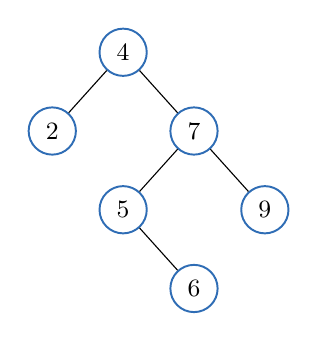
\begin{tikzpicture}[
    level distance=1cm, sibling distance=1.8cm,
    every node/.style={circle, draw=heapblue, line width=0.7pt, minimum size=6mm, inner sep=1pt, font=\small, fill=white}
]
\node {4}
    child {node {2}}
    child {node {7}
        child {node {5}
            child[missing]
            child {node {6}}
        }
        child {node {9}}
    };
\end{tikzpicture}
\end{center}

Check the property at each node:
\begin{itemize}[leftmargin=1.4em,itemsep=1pt]
    \item \textbf{Node 4:} left subtree $\{2\}$ — all $\leq 4$ $\checkmark$. Right subtree $\{5,6,7,9\}$ — all $\geq 4$ $\checkmark$.
    \item \textbf{Node 7:} left subtree $\{5,6\}$ — all $\leq 7$ $\checkmark$. Right subtree $\{9\}$ — $9 \geq 7$ $\checkmark$.
    \item \textbf{Node 5:} no left child. Right subtree $\{6\}$ — $6 \geq 5$ $\checkmark$.
    \item Leaves 2, 6, 9: no children, trivially satisfied.
\end{itemize}
\end{examplebox}

\begin{warnbox}[BST for a set $S$ is NOT unique]
The \textit{shape} of the tree depends on the \textbf{insertion order}. The same set $S = \{2,4,5,6,7,9\}$ can produce many different valid BSTs. This non-uniqueness is what leads to the worst-case problem we'll see later.
\end{warnbox}

\subsection{In-Order Traversal}

A key consequence of the BST property: visiting nodes in \textbf{left-root-right} order gives all keys in \textcolor{greenO}{ascending sorted order}.

\begin{codebox}[InOrderTraversal(x)]
\ttfamily InOrderTraversal(x):\\
\ttfamily \hspace*{2em}if x != NIL:\\
\ttfamily \hspace*{4em}InOrderTraversal(x.left) \hfill\textnormal{\itshape // recurse into left subtree}\\
\ttfamily \hspace*{4em}visit(x) \hfill\textnormal{\itshape // process current node}\\
\ttfamily \hspace*{4em}InOrderTraversal(x.right) \hfill\textnormal{\itshape // recurse into right subtree}
\end{codebox}

\textbf{Why does this produce sorted order?} The BST property guarantees: everything in the left subtree $\leq$ current node $\leq$ everything in the right subtree. Recursion applies this at every level.

\begin{examplebox}[Worked Example: In-Order Traversal]
Using the BST above (root = 4):

\begin{center}
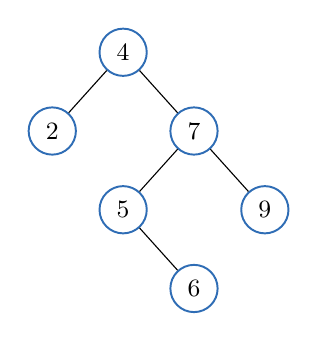
\begin{tikzpicture}[
    level distance=1cm, sibling distance=1.8cm,
    every node/.style={circle, draw=heapblue, line width=0.7pt, minimum size=6mm, inner sep=1pt, font=\small, fill=white}
]
\node {4}
    child {node {2}}
    child {node {7}
        child {node {5}
            child[missing]
            child {node {6}}
        }
        child {node {9}}
    };
\end{tikzpicture}
\end{center}

Trace: go left from 4 $\to$ visit \textbf{2} $\to$ back up, visit \textbf{4} $\to$ go right $\to$ go left from 7 $\to$ visit \textbf{5} $\to$ go right from 5 $\to$ visit \textbf{6} $\to$ back up, visit \textbf{7} $\to$ go right from 7 $\to$ visit \textbf{9}

Result: $2, 4, 5, 6, 7, 9$ \textcolor{greenO}{$\checkmark$ sorted!}
\end{examplebox}

\subsection{Left Rotation}

A \textcolor{rustW}{rotation} restructures a BST without changing which keys it stores or violating the BST property. Rotations are the fundamental tool for \textbf{rebalancing} — we'll use them heavily when we get to AVL trees next lecture.

\begin{defbox}[Left Rotation at node $x$]
Let $y = x.\text{right}$ (must exist). Left rotation at $x$:
\begin{enumerate}[leftmargin=1.4em,itemsep=2pt]
    \item $y$ takes $x$'s position (becomes new subtree root)
    \item $x$ becomes $y$'s left child
    \item $y$'s old left subtree ($B$) becomes $x$'s new right subtree
\end{enumerate}
\end{defbox}

\begin{center}
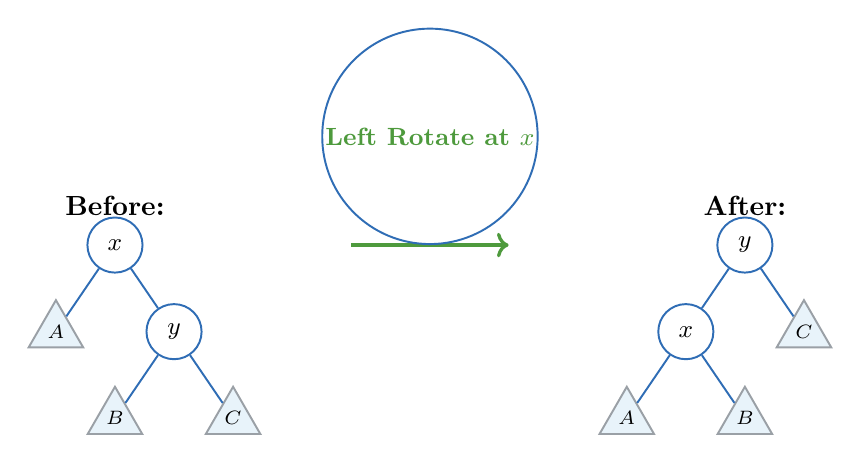
\begin{tikzpicture}[
    level distance=1.1cm, sibling distance=1.5cm,
    every node/.style={circle, draw=heapblue, line width=0.7pt, minimum size=7mm, inner sep=1pt, font=\small, fill=white},
    every child/.style={edge from parent/.style={draw=heapblue, line width=0.7pt}},
    tri/.style={regular polygon, regular polygon sides=3, draw=greyline, fill=skyfill, minimum size=8mm, inner sep=0pt, font=\scriptsize}
]
% Before
\node at (0,0.5) [draw=none, fill=none, font=\bfseries] {Before:};
\node (x) at (0,0) {$x$}
    child {node[tri] {$A$}}
    child {node (y) {$y$}
        child {node[tri] {$B$}}
        child {node[tri] {$C$}}
    };

% Arrow
\draw[->, very thick, greenO] (3,0) -- (5,0) node[midway, above, font=\small\bfseries, text=greenO] {Left Rotate at $x$};

% After
\node at (8,0.5) [draw=none, fill=none, font=\bfseries] {After:};
\node (y2) at (8,0) {$y$}
    child {node (x2) {$x$}
        child {node[tri] {$A$}}
        child {node[tri] {$B$}}
    }
    child {node[tri] {$C$}};
\end{tikzpicture}
\end{center}

\begin{keybox}[Why BST Property Is Preserved]
Before the rotation, we know: keys in $A \leq x \leq$ keys in $B \leq y \leq$ keys in $C$.

After the rotation, $B$ moves from $y$'s left to $x$'s right. But $B$'s keys are between $x$ and $y$, so $B$ being $x$'s right subtree ($\geq x$) and in $y$'s left subtree ($\leq y$) is perfectly valid. Nothing else changes.

\textcolor{violetT}{\textbf{Cost:}} $O(1)$ — just rearranging 3 pointers.
\end{keybox}

\begin{examplebox}[Worked Example: Left Rotation at Node 4]
$S = \{2, 4, 5, 6, 7, 9\}$, tree rooted at 4. Left rotate at node 4:

\textbf{Before:} root = 4, right child = 7, 7's left subtree = \{5, 6\}

\begin{center}
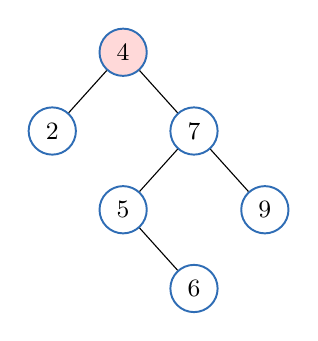
\begin{tikzpicture}[
    level distance=1cm, sibling distance=1.8cm,
    every node/.style={circle, draw=heapblue, line width=0.7pt, minimum size=6mm, inner sep=1pt, font=\small, fill=white}
]
\node[fill=red!15] {4}
    child {node {2}}
    child {node {7}
        child {node {5}
            child[missing]
            child {node {6}}
        }
        child {node {9}}
    };
\end{tikzpicture}
\hspace{1cm}
$\xrightarrow{\text{left rotate at 4}}$
\hspace{1cm}
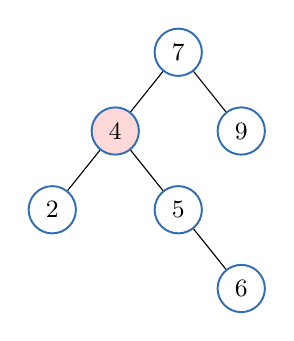
\begin{tikzpicture}[
    level distance=1cm, sibling distance=1.6cm,
    every node/.style={circle, draw=heapblue, line width=0.7pt, minimum size=6mm, inner sep=1pt, font=\small, fill=white}
]
\node {7}
    child {node[fill=red!15] {4}
        child {node {2}}
        child {node {5}
            child[missing]
            child {node {6}}
        }
    }
    child {node {9}};
\end{tikzpicture}
\end{center}

7 becomes the new root. 4 becomes 7's left child. \{5, 6\} (was 7's left subtree) becomes 4's right subtree.

\textcolor{violetT}{Verify:} In-order traversal of the result: $2, 4, 5, 6, 7, 9$. Same as before. BST property preserved. $\checkmark$
\end{examplebox}

% ==================================================================
\subsection{BST Operations}

All BST operations follow one path from root toward a leaf, making comparisons at each node to decide left or right.

\subsubsection*{Search$(T, k)$: Find a Key}

\begin{codebox}[Search(T, k)]
\ttfamily x = T.root\\
\ttfamily while x != NIL and x.key != k:\\
\ttfamily \hspace*{2em}if k < x.key:\\
\ttfamily \hspace*{4em}x = x.left \hfill\textnormal{\itshape // k must be in left subtree}\\
\ttfamily \hspace*{2em}else:\\
\ttfamily \hspace*{4em}x = x.right \hfill\textnormal{\itshape // k must be in right subtree}\\
\ttfamily return x \hfill\textnormal{\itshape // NIL if not found}
\end{codebox}

\textbf{Why this works:} The BST property tells us that if $k < x.\text{key}$, then $k$ cannot be in the right subtree (all keys there are $\geq x.\text{key} > k$). So we can safely ignore the entire right subtree and go left. Symmetric for $k > x.\text{key}$. This is the same idea as binary search on a sorted array.

\textbf{Complexity:} \textcolor{greenO}{$O(h)$} where $h$ = height of tree (we visit at most one node per level).

\begin{examplebox}[Worked Example: Search$(T, 5)$]
Tree rooted at 4 $\to$ \{2, 7 $\to$ \{5 $\to$ \{$\emptyset$, 6\}, 9\}\}:

\begin{enumerate}[leftmargin=1.4em,itemsep=1pt]
    \item At root 4: $5 > 4$ $\Rightarrow$ go \textcolor{rustW}{right} to 7
    \item At 7: $5 < 7$ $\Rightarrow$ go \textcolor{heapblue}{left} to 5
    \item At 5: $5 = 5$ $\Rightarrow$ \textcolor{greenO}{Found!} Return this node.
\end{enumerate}

3 comparisons, 3 nodes visited. Height of tree = 3, so this is within $O(h)$. $\checkmark$
\end{examplebox}

\subsubsection*{Insert$(T, z)$: Add a New Node}

\begin{codebox}[Insert(T, z)]
\ttfamily Follow the search path for z.key (comparing at each node)\\
\ttfamily When you reach a NIL position, place z there as a new leaf
\end{codebox}

\textbf{Why this works:} The search path tells us exactly where $z$ \textbf{should} be to maintain the BST property. The NIL position at the end is the only valid place for $z$'s key. Since $z$ becomes a leaf, it doesn't disturb any existing nodes.

\textbf{Complexity:} \textcolor{greenO}{$O(h)$}

\begin{examplebox}[Worked Example: Insert$(T, 10)$]
Using the same tree. Search for where 10 belongs:

\begin{enumerate}[leftmargin=1.4em,itemsep=1pt]
    \item At root 4: $10 > 4$ $\Rightarrow$ go right
    \item At 7: $10 > 7$ $\Rightarrow$ go right
    \item At 9: $10 > 9$ $\Rightarrow$ go right — but right child of 9 is NIL!
    \item \textcolor{greenO}{Insert 10 as right child of 9.}
\end{enumerate}

\begin{center}
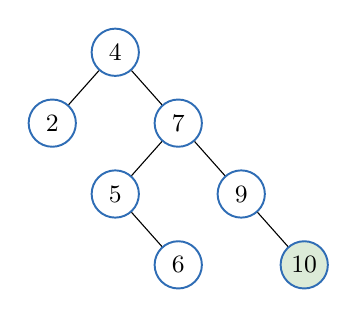
\begin{tikzpicture}[
    level distance=0.9cm, sibling distance=1.6cm,
    every node/.style={circle, draw=heapblue, line width=0.7pt, minimum size=6mm, inner sep=1pt, font=\small, fill=white}
]
\node {4}
    child {node {2}}
    child {node {7}
        child {node {5}
            child[missing]
            child {node {6}}
        }
        child {node {9}
            child[missing]
            child {node[fill=greenO!20] {10}}
        }
    };
\end{tikzpicture}
\end{center}
\end{examplebox}

% ==================================================================
\subsection{BST Delete$(T, x)$: Three Cases}

Deletion is the most complex BST operation. We have a pointer to node $x$ and need to remove it while maintaining the BST property.

\begin{warnbox}[Why deletion is tricky]
Removing a node from the middle of a tree can disconnect its children. We need to ``repair'' the tree so every node still has a parent and the BST property still holds.
\end{warnbox}

\subsubsection*{Case 1: $x$ is a leaf (no children)}

Simplest case. Just remove $x$ — nothing to reconnect.

\begin{center}
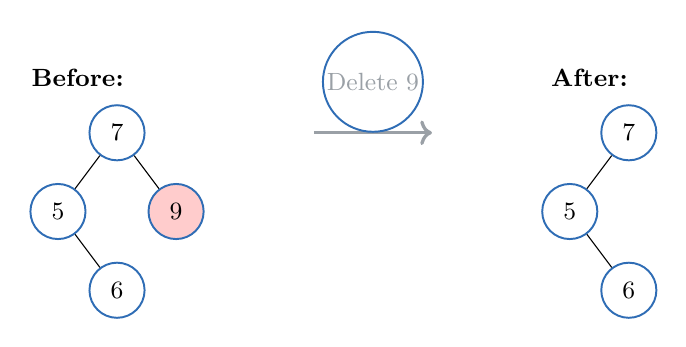
\begin{tikzpicture}[
    level distance=1cm, sibling distance=1.5cm,
    every node/.style={circle, draw=heapblue, line width=0.7pt, minimum size=7mm, inner sep=1pt, font=\small, fill=white}
]
% Before
\node at (-0.5, 0.7) [draw=none, fill=none, font=\bfseries\small] {Before:};
\node {7}
    child {node {5}
        child[missing]
        child {node {6}}
    }
    child {node[fill=red!20] {9}};

\draw[->, very thick, greyline] (2.5, 0) -- (4, 0) node[midway, above, font=\small] {Delete 9};

% After
\node at (6, 0.7) [draw=none, fill=none, font=\bfseries\small] {After:};
\node at (6.5, 0) {7}
    child {node {5}
        child[missing]
        child {node {6}}
    }
    child[missing];
\end{tikzpicture}
\end{center}

\subsubsection*{Case 2: $x$ has exactly one child}

Replace $x$ with its only child (and the child's entire subtree). The child ``moves up'' to take $x$'s position.

\textbf{Why this is safe:} if $x$ had key $k$ and its child's subtree contains keys that satisfied BST property relative to $x$, those keys also satisfy BST property relative to $x$'s parent (they were already in the correct subtree of the parent).

\begin{center}
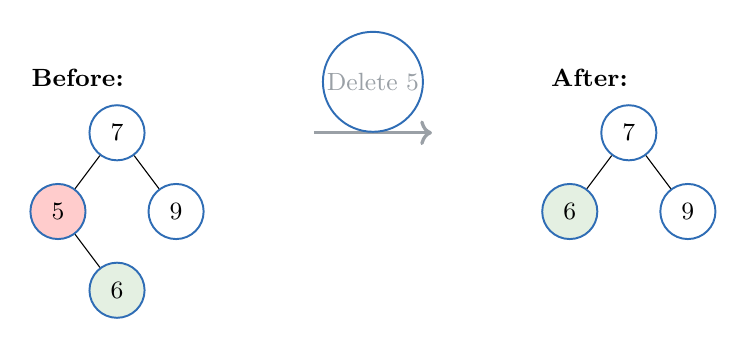
\begin{tikzpicture}[
    level distance=1cm, sibling distance=1.5cm,
    every node/.style={circle, draw=heapblue, line width=0.7pt, minimum size=7mm, inner sep=1pt, font=\small, fill=white}
]
% Before
\node at (-0.5, 0.7) [draw=none, fill=none, font=\bfseries\small] {Before:};
\node {7}
    child {node[fill=red!20] {5}
        child[missing]
        child {node[fill=greenO!15] {6}}
    }
    child {node {9}};

\draw[->, very thick, greyline] (2.5, 0) -- (4, 0) node[midway, above, font=\small] {Delete 5};

% After
\node at (6, 0.7) [draw=none, fill=none, font=\bfseries\small] {After:};
\node at (6.5, 0) {7}
    child {node[fill=greenO!15] {6}}
    child {node {9}};
\end{tikzpicture}
\end{center}

Node 6 (the only child of 5) replaces 5. BST property: $6 \leq 7$ $\checkmark$.

\subsubsection*{Case 3: $x$ has two children \textcolor{amber}{(hardest case)}}

We can't just remove $x$ — both subtrees need a parent. The solution: replace $x$'s key with its \textcolor{rustW}{successor}'s key, then delete the successor (which is easier to remove).

\begin{defbox}[The Successor]
The \textcolor{rustW}{successor} of node $x$ = the node with the \textbf{smallest key that is larger than} $x.\text{key}$.

In a BST, the successor is in $x$'s right subtree (since right subtree has all keys $\geq x.\text{key}$). To find it: go to $x$'s \textbf{right child}, then follow \textbf{left child pointers all the way down} until you hit NIL. That leftmost node in the right subtree is the successor.
\end{defbox}

\begin{keybox}[Why the Successor Has At Most One Child]
The successor is the \textbf{leftmost} node in some subtree. By definition, it has \textbf{no left child} (otherwise there would be a smaller key, contradicting ``leftmost''). So the successor has at most one child (a right child). This means deleting the successor is either Case 1 or Case 2!

This is the clever part: Case 3 \textbf{reduces to} Case 1 or 2.
\end{keybox}

\begin{enumerate}[leftmargin=1.4em,itemsep=3pt]
    \item \textbf{Find} the successor of $x$: go right once, then left all the way
    \item \textbf{Copy} the successor's key into $x$'s position (replacing $x$'s key)
    \item \textbf{Delete} the original successor node (Case 1 or 2)
\end{enumerate}

\begin{examplebox}[Worked Example: Delete$(T, 4)$ — Two Children Case (Step by Step)]
Tree: $4 \to \{2,\; 7 \to \{5 \to \{\emptyset, 6\},\; 9\}\}$

Sorted order of $S$: $2, \mathbf{4}, \textcolor{rustW}{5}, 6, 7, 9$. The \textcolor{rustW}{successor of 4 is 5}.

\bigskip

\textbf{Step 1: Find successor of 4}

\begin{center}
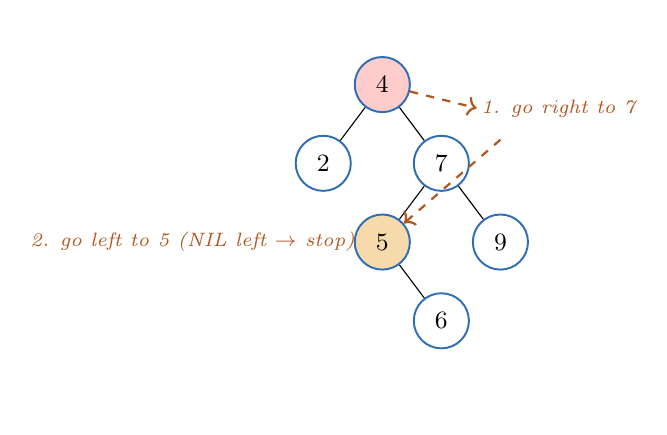
\begin{tikzpicture}[
    level distance=1cm, sibling distance=1.5cm,
    every node/.style={circle, draw=heapblue, line width=0.7pt, minimum size=7mm, inner sep=1pt, font=\small, fill=white}
]
\node[fill=red!20] (root) {4}
    child {node {2}}
    child {node {7}
        child {node[fill=goldpath!40] (succ) {5}
            child[missing]
            child {node {6}}
        }
        child {node {9}}
    };
\draw[->, thick, dashed, rustW] (root) -- ++(1.2, -0.3) node[right, draw=none, fill=none, font=\scriptsize\itshape, text=rustW] {1. go right to 7};
\draw[->, thick, dashed, rustW] (1.5, -0.7) -- (succ) node[left, draw=none, fill=none, font=\scriptsize\itshape, text=rustW, xshift=-3mm] {2. go left to 5 (NIL left $\to$ stop)};
\end{tikzpicture}
\end{center}

Go right to 7, then left to 5. Left child of 5 is NIL $\Rightarrow$ \textcolor{rustW}{successor = 5}

\bigskip

\textbf{Step 2: Copy successor's key into 4's position}

Replace 4 with 5. Now there are temporarily two nodes with key 5.

\begin{center}
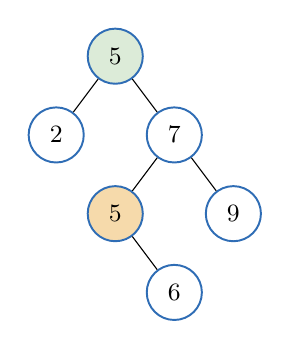
\begin{tikzpicture}[
    level distance=1cm, sibling distance=1.5cm,
    every node/.style={circle, draw=heapblue, line width=0.7pt, minimum size=7mm, inner sep=1pt, font=\small, fill=white}
]
\node[fill=greenO!20] {5}
    child {node {2}}
    child {node {7}
        child {node[fill=goldpath!40] {5}
            child[missing]
            child {node {6}}
        }
        child {node {9}}
    };
\end{tikzpicture}
\end{center}

\textbf{Step 3: Delete original successor (the highlighted 5)}

The successor node 5 has one child (6) $\Rightarrow$ \textcolor{rustW}{Case 2}. Replace the successor 5 with its child 6:

\begin{center}
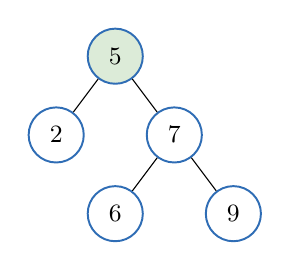
\begin{tikzpicture}[
    level distance=1cm, sibling distance=1.5cm,
    every node/.style={circle, draw=heapblue, line width=0.7pt, minimum size=7mm, inner sep=1pt, font=\small, fill=white}
]
\node[fill=greenO!20] {5}
    child {node {2}}
    child {node {7}
        child {node {6}}
        child {node {9}}
    };
\end{tikzpicture}
\end{center}

\textbf{Final result:} $5 \to \{2,\; 7 \to \{6, 9\}\}$

\textcolor{violetT}{Verify in-order:} $2, 5, 6, 7, 9$ $\checkmark$ (4 removed, BST property intact)
\end{examplebox}

\begin{examplebox}[Practice Problem: BST Delete]
\textbf{Q:} Given BST: $8 \to \{3 \to \{1, 6 \to \{4, 7\}\},\; 10 \to \{\emptyset, 14 \to \{13, \emptyset\}\}\}$

Delete node 3 (two children).

\begin{answerband}
\textbf{Solution:}
\begin{enumerate}[leftmargin=1.4em,itemsep=1pt]
    \item Successor of 3: go right to 6, then all-way left to 4. Successor = 4.
    \item Copy 4 into 3's position.
    \item Delete original 4: it is a leaf (Case 1), just remove it.
    \item Result: $8 \to \{4 \to \{1, 6 \to \{\emptyset, 7\}\},\; 10 \to \{\emptyset, 14 \to \{13, \emptyset\}\}\}$
\end{enumerate}

In-order: $1, 4, 6, 7, 8, 10, 13, 14$ $\checkmark$
\end{answerband}
\end{examplebox}

\begin{keybox}[BST Delete: Summary of All 3 Cases]
\begin{center}
\renewcommand{\arraystretch}{1.5}
\begin{tabular}{c l l}
\textbf{Case} & \textbf{Condition} & \textbf{Action} \\
\hline
1 & $x$ is a \textcolor{rustW}{leaf} (0 children) & Remove $x$ \\
2 & $x$ has \textcolor{rustW}{one child} & Replace $x$ with that child \\
3 & $x$ has \textcolor{rustW}{two children} & Copy successor's key into $x$, delete successor (Case 1 or 2) \\
\end{tabular}
\end{center}

\textbf{All cases:} \textcolor{greenO}{$O(h)$}. Finding successor walks down at most $h$ nodes. Removing the successor is $O(1)$.
\end{keybox}

% ==================================================================
\subsection{The Problem: Worst-Case Height}

All BST operations run in $O(h)$ where $h$ = height of the tree. So the real question is: \textbf{how tall can a BST get?}

\textbf{Best case:} A perfectly balanced BST with $n$ nodes has height $\lfloor \log_2 n \rfloor$. All operations are $O(\log n)$.

\textbf{Worst case:} Consider inserting $1, 2, 3, \ldots, n$ \textbf{in sorted order}:

\begin{itemize}[leftmargin=1.4em,itemsep=2pt]
    \item Insert 1: root = 1
    \item Insert 2: $2 > 1$, goes right. Now: $1 \to 2$
    \item Insert 3: $3 > 1$, right. $3 > 2$, right. Now: $1 \to 2 \to 3$
    \item $\vdots$
    \item Insert $n$: goes right at every step. Chain: $1 \to 2 \to 3 \to \cdots \to n$
\end{itemize}

\begin{center}
\begin{tikzpicture}[
    every node/.style={circle, draw=heapblue, line width=0.7pt, minimum size=6mm, inner sep=1pt, font=\small, fill=white}
]
\node (n1) at (0, 0) {1};
\node (n2) at (0.8, -0.8) {2};
\node (n3) at (1.6, -1.6) {3};
\node (dots) at (2.2, -2.2) [draw=none, fill=none] {$\ddots$};
\node (nn) at (2.8, -2.8) {$n$};
\draw[heapblue, line width=0.7pt] (n1) -- (n2);
\draw[heapblue, line width=0.7pt] (n2) -- (n3);
\draw[heapblue, dashed] (n3) -- (dots);
\draw[heapblue, dashed] (dots) -- (nn);
\node[draw=none, fill=none, font=\small\color{rustW}] at (4.5, -1.4) {height $= n - 1$};
\end{tikzpicture}
\end{center}

This is a \textcolor{rustW}{degenerate chain} — every node has exactly one child. It is a valid BST but it looks like a linked list!

\textbf{Height} $= n - 1$ edges. So all operations become $\Theta(n)$:

\begin{center}
\renewcommand{\arraystretch}{1.4}
\begin{tabular}{l c c}
& \textbf{Best-case BST} & \textbf{Worst-case BST} \\
\hline
Search & $O(\log n)$ & \textcolor{rustW}{$\Theta(n)$} \\
Insert & $O(\log n)$ & \textcolor{rustW}{$\Theta(n)$} \\
Delete & $O(\log n)$ & \textcolor{rustW}{$\Theta(n)$} \\
\end{tabular}
\end{center}

\begin{warnbox}[Plain BSTs are not good enough!]
A plain BST gives us no guarantee on height. If the input happens to be sorted (or nearly sorted), we degrade to a linked list. We need a BST variant that \textbf{automatically rebalances} to keep the height small.
\end{warnbox}

\textcolor{violetT}{\textbf{Next lecture:}} the \textcolor{rustW}{AVL tree} — a self-balancing BST that guarantees height $\leq$ \textcolor{greenO}{$O(\log n)$}, making all dictionary operations $O(\log n)$ in the \textbf{worst case}. It uses \textbf{rotations} (like the left rotation we just learned) to rebalance after every insert and delete.

% ==================================================================
\section{Past Exam Questions}

\begin{exambox}[Seen on a past exam \textnormal{(Fall 2014 Midterm, Q3b)}]

\textbf{[4 marks]} Draw the result when \textbf{55 is deleted} from the AVL tree below. Show your work; in particular, identify clearly any \textbf{rotation} performed.

\begin{center}
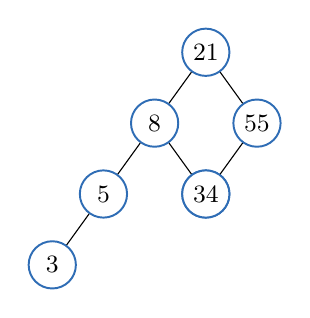
\begin{tikzpicture}[
    level distance=0.9cm, sibling distance=1.3cm,
    every node/.style={circle, draw=heapblue, line width=0.7pt, minimum size=6mm, inner sep=1pt, font=\small, fill=white}
]
\node {21}
    child {node {8}
        child {node {5}
            child {node {3}}
            child[missing]
        }
        child {node {13}}
    }
    child {node {55}
        child {node {34}}
        child[missing]
    };
\end{tikzpicture}
\end{center}

\begin{answerband}
\textbf{Step 1: BST-Delete 55.} Node 55 has one child (34) $\Rightarrow$ Case 2: replace 55 with 34.

Result: $21 \to \{8 \to \{5 \to \{3, \emptyset\}, 13\}, 34\}$

\textbf{Step 2: Check AVL balance.} Node 21 has left subtree height 2, right subtree height 0. Balance factor $= |2 - 0| = 2 > 1$. \textcolor{rustW}{Unbalanced!}

\textbf{Step 3: Rotate.} Right-rotate at 21 (with 8 as pivot).

Final result: $8 \to \{5 \to \{3, \emptyset\}, 21 \to \{13, 34\}\}$

\medskip
\textcolor{violetT}{\textbf{Key concepts tested:}} BST Delete (Case 2) + AVL balance check + Rotation.

\textit{(AVL trees are covered in Lecture 5. This exam question is included to show what's coming and how BST deletion connects to AVL rebalancing.)}
\end{answerband}
\end{exambox}

\begin{exambox}[Seen on a past exam \textnormal{(Fall 2014 Midterm, Q2)}]
\textbf{[10 marks]} Consider the ``k-Set'' ADT:

\textbf{Objects:} Collection $C$ of rational numbers (duplicates allowed).

\textbf{Operations:}
\begin{itemize}[leftmargin=1.4em,itemsep=1pt]
    \item \texttt{Insert$(C, x)$}: add $x$ to $C$
    \item \texttt{k-Select$(C)$}: return element at rank $k$ in $C$, or NIL if $|C| < k$
\end{itemize}

Implement using data structures from class. \texttt{k-Select} must run in \textcolor{greenO}{$O(1)$} worst case.

\begin{answerband}
\textbf{Solution:} Store $k$ smallest elements in a \textcolor{rustW}{max-heap} $H_1$, rest in \textcolor{rustW}{min-heap} $H_2$.

\textbf{Idea:} the $k$-th smallest element = the largest among the $k$ smallest = root of a max-heap containing exactly the $k$ smallest.

\texttt{k-Select$(C)$}: if $|H_1| < k$: return NIL; else return $H_1[1]$ (root of max-heap). $O(1)$.

\texttt{Insert$(C, x)$}: if $x < H_1[1]$ or $|H_1| < k$: insert into $H_1$, else insert into $H_2$. If $|H_1| > k$: extract max from $H_1$, insert into $H_2$. Cost: \textcolor{greenO}{$O(\log n)$}.

\medskip
\textcolor{violetT}{\textbf{Key concepts tested:}} Heap operations, ADT implementation, runtime analysis
\end{answerband}
\end{exambox}

% ==================================================================
\section*{\textcolor{violetT}{Quick Reference: Lecture 4}}
\addcontentsline{toc}{section}{Quick Reference: Lecture 4}
\begin{keybox}
\renewcommand{\arraystretch}{1.4}
\begin{tabular}{l l}
\multicolumn{2}{l}{\textbf{\textcolor{utnavy}{Binomial Heaps (Part 2)}}}\\
Decrease\_Key & set key, bubble up via PARENT pointer $\to$ $O(\log n)$\\
Delete & Decrease\_Key($-\infty$) + Extract\_Min $\to$ $O(\log n)$\\
Increase\_Key & Delete + Insert (not bubble-down: that's $O(\log^2 n)$) $\to$ $O(\log n)$\\
$k$ inserts total cost & $k + \alpha(n) - \alpha(n+k)$; $\leq 2k$ when $k > \log_2 n$\\
Average insert cost & $< 2$ key comparisons (when $k > \log_2 n$)\\[6pt]
\multicolumn{2}{l}{\textbf{\textcolor{utnavy}{Dictionary ADT + BST}}}\\
Dictionary ADT & Search + Insert + Delete on keyed elements\\
Linked list baseline & Insert $\Theta(1)$, Search/Delete $\Theta(n)$\\
BST property & left subtree keys $\leq$ node key $\leq$ right subtree keys\\
In-order traversal & left $\to$ visit $\to$ right = sorted order\\
Left rotation & $x$ goes down, $x.\text{right}$ goes up; preserves BST; $O(1)$\\
BST Search/Insert & follow comparisons down the tree; $O(h)$\\
BST Delete & 3 cases: leaf / 1 child / 2 children (via successor); $O(h)$\\
Worst-case BST height & $n - 1$ (degenerate chain) $\Rightarrow$ all ops $\Theta(n)$\\
\textbf{Next: AVL trees} & guarantee height $O(\log n)$ via rotations\\
\end{tabular}
\end{keybox}

\vspace{4pt}

% ******************************************************************
%  PASTE INSTRUCTIONS:
%
%  1. In your master document, DELETE these 3 lines near the end:
%       \begin{center}\textcolor{greyline}{\rule{0.5\linewidth}{0.6pt}}\end{center}
%       \begin{center}\small\textcolor{greyline}{End of Lectures 1, 2, 3 \& 4 notes.}\end{center}
%       \end{document}
%
%  2. Paste EVERYTHING below this comment block in their place.
%
%  3. On the cover page, change:
%       {\large\textcolor{violetT}{Lectures 1, 2, 3 \& 4}}
%     to:
%       {\large\textcolor{violetT}{Lectures 1, 2, 3, 4 \& 5}}
%
%  That's it. No preamble changes needed.
% ******************************************************************

\newpage

% ******************************************************************
%  PART V: LECTURE 5 — AVL TREES (PART 1)
% ******************************************************************

\part*{\textcolor{utnavy}{Lecture 5: Balanced BSTs and AVL Trees}}
\addcontentsline{toc}{part}{Lecture 5: Balanced BSTs and AVL Trees}

% ==================================================================
\section{Recall: the Problem with BSTs}

A plain BST implements the \textbf{Dictionary ADT} (Search, Insert, Delete), each in \textcolor{greenO}{$\Theta(h)$} where $h$ is the height. The catch: if we insert keys in sorted order $1, 2, 3, \ldots, n$, the tree becomes a \textcolor{rustW}{degenerate chain} with height $\Theta(n)$, so every operation is $\Theta(n)$.

\begin{keybox}[Goal]
Keep the tree \textbf{balanced} so its height stays \textcolor{greenO}{$\Theta(\log n)$}. Then Search, Insert, Delete are all \textcolor{greenO}{$\Theta(\log n)$}.
\end{keybox}

\textbf{Balanced BST} data structures for the Dictionary ADT: \textcolor{heapblue}{2-3 trees}, \textcolor{heapblue}{Red-Black trees}, \textcolor{heapblue}{B-Trees}, and \textcolor{rustW}{AVL trees} (this lecture).

% ==================================================================
\section{Reminder: Height of a Node}

\begin{defbox}[Height]
$\text{height}(v)$ = number of \textcolor{rustW}{edges} on the longest path from $v$ down to a leaf.
\begin{itemize}[leftmargin=1.4em,itemsep=1pt]
  \item $\text{height}(v) = 0$ \quad if $v$ is a \textbf{leaf} (a single node).
  \item $\text{height}(\text{empty tree}) = -1$.
\end{itemize}
$\text{height}(T)$ = height of the root node of $T$.
\end{defbox}

The $-1$ for the empty tree is a convention that makes the recurrence $\text{height}(v) = 1 + \max(\text{height}(v.\text{left}),\, \text{height}(v.\text{right}))$ work even when a child is missing.

% ==================================================================
\section{Balance Factor (BF)}

\begin{defbox}[Balance Factor of a node $v$]
\begin{center}\large
$\text{BF}(v) \;=\; \text{height}(\text{right subtree of } v) \;-\; \text{height}(\text{left subtree of } v) \;=\; h_R - h_L$
\end{center}
\end{defbox}

The bigger $|\text{BF}(v)|$, the more \textcolor{rustW}{imbalanced} the node. We want every $\text{BF}(v)$ as close to $0$ as possible.

\begin{keybox}[Reading the Balance Factor]
\renewcommand{\arraystretch}{1.4}
\begin{tabular}{c l}
$\text{BF}(v) = \textcolor{rustW}{+1}$ & $v$ is \textcolor{rustW}{\textbf{right-heavy}} \; ($h_R = h_L + 1$)\\
$\text{BF}(v) = \textcolor{greenO}{\phantom{+}0}$ & $v$ is \textcolor{greenO}{\textbf{balanced}} \; ($h_R = h_L$)\\
$\text{BF}(v) = \textcolor{heapblue}{-1}$ & $v$ is \textcolor{heapblue}{\textbf{left-heavy}} \; ($h_L = h_R + 1$)\\
\end{tabular}
\end{keybox}

% ==================================================================
\section{AVL Tree Definition (Adelson-Velsky and Landis)}

\begin{defbox}[\textcolor{defblue}{AVL Tree (MUST KNOW)}]
An \textbf{AVL tree} $T$ is a BST where \textbf{every} node $v \in T$ satisfies
\begin{center}\Large
$-1 \;\;\textcolor{rustW}{\leq}\;\; \text{BF}(v) \;\;\textcolor{rustW}{\leq}\;\; +1$
\end{center}
Every node is left-heavy, balanced, or right-heavy. \textbf{No node may reach $\pm 2$.}
\end{defbox}

% ==================================================================
\section{Is This an AVL Tree?}

To check: compute $\text{BF}(v)$ at \emph{every} node. It is an AVL tree \textbf{iff} every $|\text{BF}(v)| \leq 1$. A single node with $|\text{BF}| \geq 2$ breaks it.

\begin{examplebox}[One tree, balance factor on every node]
Compute $h_R - h_L$ at each node (heights shown are of the subtree rooted there).

\begin{center}
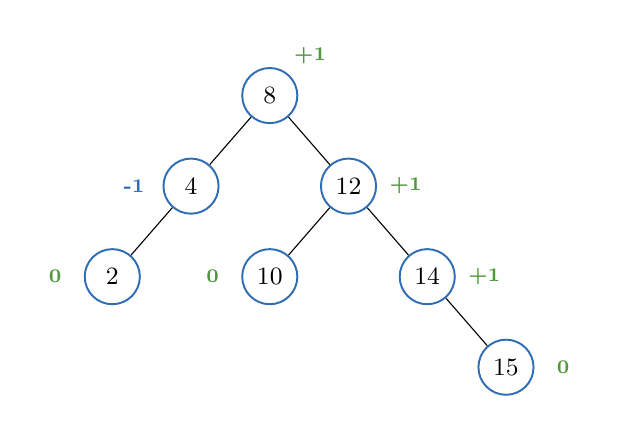
\begin{tikzpicture}[
    level distance=1.15cm, sibling distance=2.0cm,
    every node/.style={circle, draw=heapblue, line width=0.7pt, minimum size=7mm, inner sep=1pt, font=\small, fill=white}
]
\node [label={[greenO,font=\scriptsize\bfseries]above right:{+1}}] {8}
    child {node [label={[heapblue,font=\scriptsize\bfseries]left:{-1}}] {4}
        child {node [label={[greenO,font=\scriptsize\bfseries]left:{0}}] {2}}
        child[missing]
    }
    child {node [label={[greenO,font=\scriptsize\bfseries]right:{+1}}] {12}
        child {node [label={[greenO,font=\scriptsize\bfseries]left:{0}}] {10}}
        child {node [label={[greenO,font=\scriptsize\bfseries]right:{+1}}] {14}
            child[missing]
            child {node [label={[greenO,font=\scriptsize\bfseries]right:{0}}] {15}}
        }
    };
\end{tikzpicture}
\end{center}

Every $|\text{BF}| \leq 1$, so this \textbf{is} an AVL tree. \textcolor{greenO}{$\checkmark$}
\end{examplebox}

\begin{warnbox}[When it is NOT an AVL tree]
If any node reaches $\text{BF} = \textcolor{rustW}{+2}$ or $\text{BF} = \textcolor{rustW}{-2}$, the tree is not AVL. Example: a node whose left subtree has height $0$ and right subtree has height $2$ gives $\text{BF} = 2 - 0 = +2$. \textcolor{rustW}{Not AVL.}
\end{warnbox}

% ==================================================================
\section{Properties of AVL Trees}

\begin{keybox}[Why AVL trees are good]
\begin{itemize}[leftmargin=1.4em,itemsep=2pt]
  \item An AVL tree of $n$ nodes has height \textcolor{violetT}{$\Theta(\log n)$} \quad\big[precisely, $\text{height} \leq 1.44\,\log_2(n+2)$\big].
  \item Insert and Delete can maintain the balance in \textcolor{violetT}{$\Theta(\log n)$} time.
  \item Elegant, relatively clean and simple, works well in practice.
\end{itemize}
So Search, Insert, Delete are all \textcolor{greenO}{$\Theta(\log n)$} worst case.
\end{keybox}

\begin{exambox}[Seen on a past exam \textnormal{(Fall 2014 Midterm, Q3a)}]
\textbf{[4 marks]} Draw an AVL tree containing $\{1, 2, \ldots, 12\}$, but make it \textbf{as unbalanced as possible}. Next to each node, indicate the \textbf{height} of the subtree rooted at that node.

\begin{answerband}
``As unbalanced as possible'' = the \textbf{minimum} number of nodes are used to reach the height, so every node sits at its balance limit ($\text{BF} = \pm 1$). One valid answer (height shown as a subscript):

\begin{center}
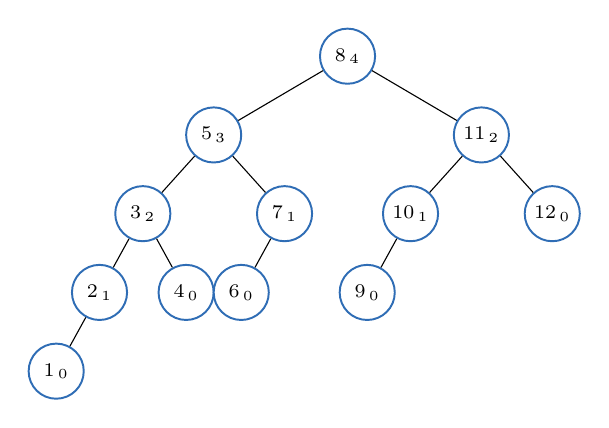
\begin{tikzpicture}[
    level distance=1.0cm,
    every node/.style={circle, draw=heapblue, line width=0.7pt, minimum size=7mm, inner sep=1pt, font=\scriptsize, fill=white},
    level 1/.style={sibling distance=3.4cm},
    level 2/.style={sibling distance=1.8cm},
    level 3/.style={sibling distance=1.1cm}
]
\node {$8_{\,4}$}
  child {node {$5_{\,3}$}
    child {node {$3_{\,2}$}
      child {node {$2_{\,1}$}
        child {node {$1_{\,0}$}}
        child[missing]
      }
      child {node {$4_{\,0}$}}
    }
    child {node {$7_{\,1}$}
      child {node {$6_{\,0}$}}
      child[missing]
    }
  }
  child {node {$11_{\,2}$}
    child {node {$10_{\,1}$}
      child {node {$9_{\,0}$}}
      child[missing]
    }
    child {node {$12_{\,0}$}}
  };
\end{tikzpicture}
\end{center}

\textcolor{violetT}{\textbf{Key idea:}} The subtree of height $4$ (root $8$) uses one child of height $3$ and, by the AVL rule, the other child may be as short as height $2$. That is the fewest nodes possible, which is why it looks so lopsided while still being AVL.
\end{answerband}
\end{exambox}

\begin{exambox}[Seen on a past exam \textnormal{(Fall 2014 Midterm, Q3c)}]
\textbf{[4 marks]} Let $m(h)$ = the \textbf{minimum} number of nodes in any AVL tree of height $h$. Give a recurrence for $m(h)$ with base cases, and explain it briefly.

\begin{answerband}
\[
  m(0) = 1, \qquad m(1) = 2, \qquad m(h) = 1 + m(h-1) + m(h-2) \;\; \text{for } h \geq 2.
\]
\textbf{Why:} height $0$ needs $1$ node; height $1$ needs a root with one child ($2$ nodes). For height $h$, the root ($1$ node) needs one child of height $h-1$; by the AVL condition the \emph{other} child can be as short as height $h-2$. Making both children minimal gives $m(h-1) + m(h-2)$ below the root.

\smallskip
\textcolor{violetT}{\textbf{Consequence:}} $m(h)$ grows like the Fibonacci numbers (exponentially in $h$), which forces $h = \Theta(\log n)$. This is the proof that AVL height is logarithmic.
\end{answerband}
\end{exambox}

% ==================================================================
\section{AVL Operations}

\begin{keybox}[The three operations]
\renewcommand{\arraystretch}{1.4}
\begin{tabular}{l l}
\textcolor{heapblue}{\textbf{Search}$(T, x)$} & identical to BST search $\to$ \textcolor{greenO}{$O(\log n)$} (height is $O(\log n)$)\\
\textcolor{heapblue}{\textbf{Insert}$(T, x)$} & BST insert $+$ rebalance $\to$ \textcolor{violetT}{$O(\log n)$}\\
\textcolor{heapblue}{\textbf{Delete}$(T, x)$} & BST delete $+$ rebalance $\to$ \textcolor{violetT}{$O(\log n)$}\\
\end{tabular}
\end{keybox}

Search is unchanged from a plain BST, so the only new work is keeping the tree balanced after Insert (and Delete). This lecture covers \textbf{Insert}.

% ==================================================================
\section{Insert: General Idea}

\begin{keybox}[Insert$(T, x)$: the plan]
\begin{enumerate}[leftmargin=1.6em,itemsep=2pt]
  \item Insert $x$ into $T$ as in any BST. Now $x$ is a \textbf{leaf}; set $\text{BF}(x) = 0$.
  \item Walk \textbf{from $x$ up to the root}. Only the balance factors of nodes \emph{on this path} can change.
  \item At each node $v$ on the path, \textbf{adjust} $\text{BF}(v)$. If some $v$ becomes $\pm 2$, \textbf{rebalance} at $v$ with a rotation.
\end{enumerate}
\end{keybox}

\textbf{Why only the path changes:} inserting a leaf only lengthens paths that pass through $x$'s ancestors. No other node's subtree heights move.

\begin{keybox}[The stopping rule]
Going up, at each ancestor $v$:
\begin{itemize}[leftmargin=1.4em,itemsep=1pt]
  \item If the subtree containing $x$ got taller, $\text{BF}(v)$ moves by $\pm 1$.
  \item \textbf{If $\text{BF}(v)$ becomes $0$}, the subtree at $v$ did \emph{not} grow taller overall $\Rightarrow$ \textcolor{greenO}{stop}. Nothing above $v$ can change.
  \item If $\text{BF}(v)$ becomes $\pm 2$, rotate to fix it (then the height is restored, so we also stop).
\end{itemize}
\end{keybox}

% ==================================================================
\section{Worked Example 1: Insert with No Rebalancing}

Start from this AVL tree of $\{1, 3, 7, 12, 14, 17, 19\}$ (all $\text{BF} = 0$), and \textbf{Insert 8}.

\begin{center}
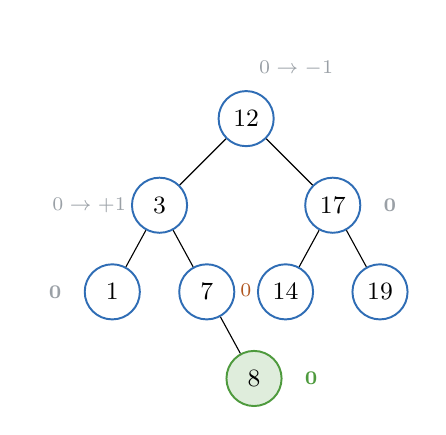
\begin{tikzpicture}[
    level distance=1.1cm, sibling distance=2.2cm,
    every node/.style={circle, draw=heapblue, line width=0.7pt, minimum size=7mm, inner sep=1pt, font=\small, fill=white},
    level 2/.style={sibling distance=1.2cm}
]
\node [label={[greyline,font=\scriptsize\bfseries]above right:{$0\to-1$}}] {12}
    child {node [label={[greyline,font=\scriptsize\bfseries]left:{$0\to+1$}}] {3}
        child {node [label={[greyline,font=\scriptsize\bfseries]left:{0}}] {1}}
        child {node [label={[rustW,font=\scriptsize\bfseries]right:{$0\to+1$}}] {7}
            child[missing]
            child {node[fill=greenO!18,draw=greenO] [label={[greenO,font=\scriptsize\bfseries]right:{0}}] {8}}
        }
    }
    child {node [label={[greyline,font=\scriptsize\bfseries]right:{0}}] {17}
        child {node {14}}
        child {node {19}}
    };
\end{tikzpicture}
\end{center}

\begin{examplebox}[Trace: Insert 8]
\begin{enumerate}[leftmargin=1.4em,itemsep=2pt]
  \item BST-insert $8$: it lands as the \textbf{right child of 7}. Set $\text{BF}(8) = 0$.
  \item Go up to $7$: $8$ is in $7$'s right subtree $\Rightarrow$ $\text{BF}(7): 0 \to +1$. Still legal, and \textbf{the height of the subtree at 7 did not change} (it was $1$ before, it is still $1$). \textcolor{rustW}{So we stop at 7.}
\end{enumerate}
\textcolor{violetT}{\textbf{Because the height of 7's subtree is unchanged, no ancestor above it is affected}} (3 and 12 keep their old balance factors, shown greyed). \textcolor{greenO}{No rebalancing needed.}
\end{examplebox}

\begin{warnbox}[Watch the ``+1 at 3'' question]
After inserting $8$, node $3$ would only change if $7$'s subtree grew. It did not, so we never even reach $3$: we stop the moment a node keeps its height. This is the whole point of the stopping rule.
\end{warnbox}

% ==================================================================
\section{Worked Example 2: Single Rotation (Left Rotation)}

Now the tree is the AVL of $\{1, 3, 5, 7, 8, 12, 14, 17, 19\}$. \textbf{Insert 10.}

$10$ BST-inserts as the \textbf{right child of 8}. Walking up: $\text{BF}(8): 0 \to +1$, then $\text{BF}(7): 0 \to +1$, then $\text{BF}(3): +1 \to \textcolor{rustW}{+2}$. \textcolor{rustW}{Node 3 is now unbalanced (right-heavy), and its right child 7 is also right-heavy ($+1$).}

\begin{keybox}[This is the ``right-right'' (RR) case $\Rightarrow$ single Left Rotation]
$v = 3$ has $\text{BF}(v) = +2$ \textbf{and} $\text{BF}(v.\text{right}) = +1$. Fix with one \textbf{Left Rotation} at $v$.
\end{keybox}

\begin{center}
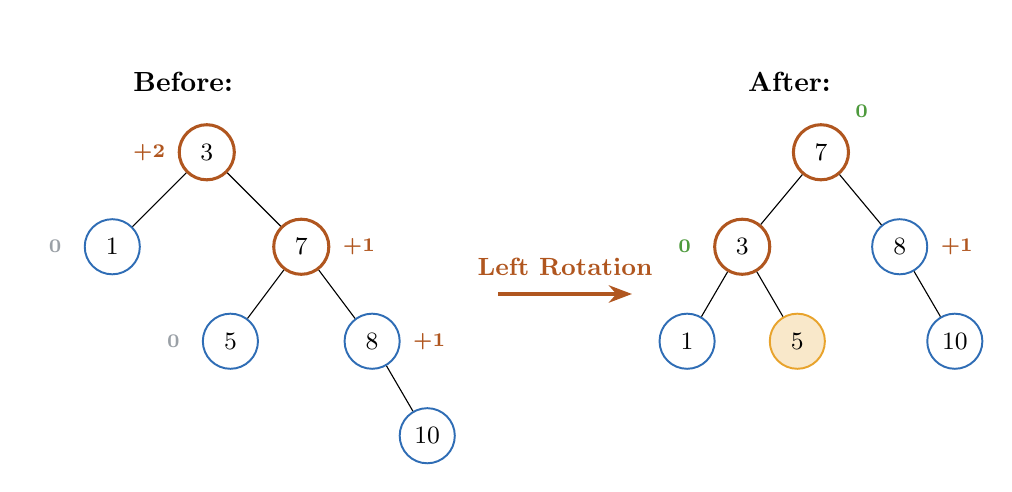
\begin{tikzpicture}[
    every node/.style={circle, draw=heapblue, line width=0.7pt, minimum size=7mm, inner sep=1pt, font=\small, fill=white}
]
% ---- BEFORE (left) ----
\node[font=\bfseries, draw=none, fill=none] at (0.3,0.9) {Before:};
\node[draw=rustW,line width=1.1pt, label={[rustW,font=\scriptsize\bfseries]left:{+2}}] (b3) at (0.6,0) {3};
\node[label={[greyline,font=\scriptsize\bfseries]left:{0}}] (b1) at (-0.6,-1.2) {1};
\node[draw=rustW,line width=1.1pt, label={[rustW,font=\scriptsize\bfseries]right:{+1}}] (b7) at (1.8,-1.2) {7};
\node[label={[greyline,font=\scriptsize\bfseries]left:{0}}] (b5) at (0.9,-2.4) {5};
\node[label={[rustW,font=\scriptsize\bfseries]right:{+1}}] (b8) at (2.7,-2.4) {8};
\node (b10) at (3.4,-3.6) {10};
\draw (b3)--(b1); \draw (b3)--(b7); \draw (b7)--(b5); \draw (b7)--(b8); \draw (b8)--(b10);

% ---- arrow ----
\draw[-{Stealth}, line width=1.2pt, rustW] (4.3,-1.8) -- (6.0,-1.8);
\node[rustW,font=\small\bfseries, draw=none, fill=none] at (5.15,-1.45) {Left Rotation};

% ---- AFTER (right) ----
\node[font=\bfseries, draw=none, fill=none] at (8.0,0.9) {After:};
\node[draw=rustW,line width=1.1pt, label={[greenO,font=\scriptsize\bfseries]above right:{0}}] (a7) at (8.4,0) {7};
\node[draw=rustW,line width=1.1pt, label={[greenO,font=\scriptsize\bfseries]left:{0}}] (a3) at (7.4,-1.2) {3};
\node[label={[rustW,font=\scriptsize\bfseries]right:{+1}}] (a8) at (9.4,-1.2) {8};
\node (a1) at (6.7,-2.4) {1};
\node[fill=goldpath!25,draw=goldpath] (a5) at (8.1,-2.4) {5};
\node (a10) at (10.1,-2.4) {10};
\draw (a7)--(a3); \draw (a7)--(a8); \draw (a3)--(a1); \draw (a3)--(a5); \draw (a8)--(a10);
\end{tikzpicture}
\end{center}

\begin{examplebox}[Reading the rotation]
Left-rotating at $3$: its right child $7$ becomes the new subtree root, and $3$ becomes $7$'s \textbf{left} child.
\begin{itemize}[leftmargin=1.4em,itemsep=2pt]
  \item \textbf{Where does 5 go?} $5$ was $7$'s \emph{left} subtree. In a left rotation, $7$'s old left subtree becomes $3$'s new \textbf{right} subtree. So \textcolor{goldpath}{$5$ hangs under $3$, not under $8$}, because $3 < 5 < 7$, so $5$ belongs on $3$'s right. (BST property preserved.)
  \item After: $\text{BF}(7) = 0$, so $7$'s subtree is balanced again.
\end{itemize}
\end{examplebox}

\begin{keybox}[Bonus: nothing propagates upward]
The subtree rooted at $3$ had height $2$ \emph{before} inserting $10$; after the rotation the subtree rooted at $7$ has height $2$ again. \textbf{Same height as before the insert}, so the balance factor of $12$ (the parent) is unchanged and we \textcolor{greenO}{stop}. One rotation fixes everything.
\end{keybox}

% ==================================================================
\section{Worked Example 3: Double Rotation (Right-Left)}

Tree is the AVL of $\{1, 3, 5, 7, 8, 12, 14, 17, 19\}$. \textbf{Insert 6.}

$6$ BST-inserts as the \textbf{right child of 5}. Walking up: $\text{BF}(5): 0 \to +1$, $\text{BF}(7): 0 \to \textcolor{heapblue}{-1}$, $\text{BF}(3): +1 \to \textcolor{rustW}{+2}$. Now $v = 3$ has $\text{BF} = +2$, but its right child $7$ is \textcolor{heapblue}{left-heavy ($-1$)}: the ``bend'' zig-zags.

\begin{warnbox}[A single Left Rotation does NOT fix this]
Because the heavy grandchild is on the \emph{left} of the right child (a right-then-left zig-zag), one left rotation at $3$ leaves the tree unbalanced. We need \textbf{two} rotations.
\end{warnbox}

\begin{keybox}[This is the ``right-left'' (RL) case $\Rightarrow$ Double Right-Left Rotation]
$v = 3$ has $\text{BF}(v) = +2$ \textbf{and} $\text{BF}(v.\text{right}) = -1$.
\begin{enumerate}[leftmargin=1.6em,itemsep=1pt]
  \item \textbf{Right-rotate} the right subtree of $v$ (rotate around $7$).
  \item \textbf{Left-rotate} at $v$ (rotate around $3$).
\end{enumerate}
\end{keybox}

\begin{center}
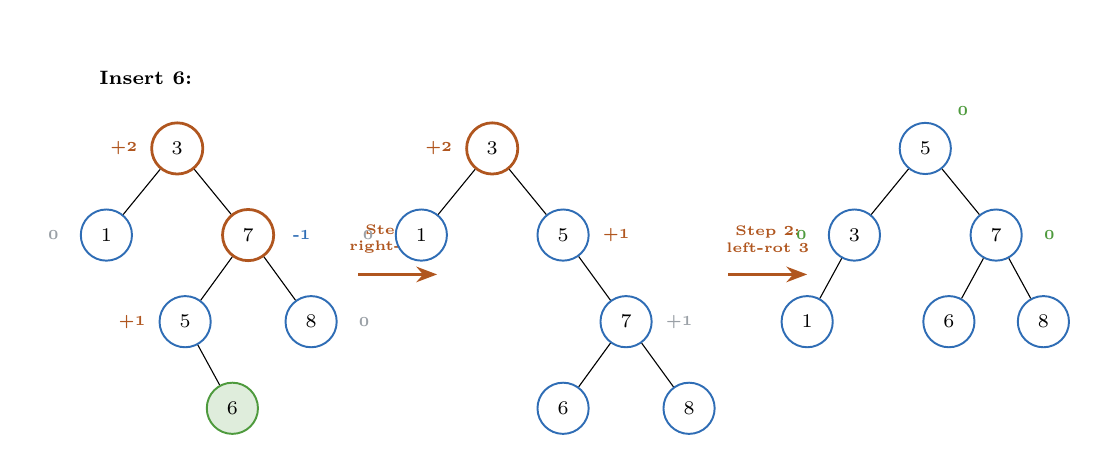
\begin{tikzpicture}[
    every node/.style={circle, draw=heapblue, line width=0.7pt, minimum size=6.5mm, inner sep=1pt, font=\scriptsize, fill=white}
]
% ---- START ----
\node[font=\bfseries\scriptsize, draw=none, fill=none] at (0.0,0.9) {Insert 6:};
\node[draw=rustW,line width=1pt, label={[rustW,font=\tiny\bfseries]left:{+2}}] (s3) at (0.4,0) {3};
\node[label={[greyline,font=\tiny\bfseries]left:{0}}] (s1) at (-0.5,-1.1) {1};
\node[draw=rustW,line width=1pt, label={[heapblue,font=\tiny\bfseries]right:{-1}}] (s7) at (1.3,-1.1) {7};
\node[label={[rustW,font=\tiny\bfseries]left:{+1}}] (s5) at (0.5,-2.2) {5};
\node[label={[greyline,font=\tiny\bfseries]right:{0}}] (s8) at (2.1,-2.2) {8};
\node[fill=greenO!18,draw=greenO] (s6) at (1.1,-3.3) {6};
\draw (s3)--(s1); \draw (s3)--(s7); \draw (s7)--(s5); \draw (s7)--(s8); \draw (s5)--(s6);

% arrow 1
\draw[-{Stealth}, line width=1pt, rustW] (2.7,-1.6) -- (3.7,-1.6);
\node[rustW,font=\tiny\bfseries, draw=none, fill=none, align=center] at (3.2,-1.15) {Step 1:\\ right-rot 7};

% ---- MIDDLE (after right-rotate around 7) ----
\node[draw=rustW,line width=1pt, label={[rustW,font=\tiny\bfseries]left:{+2}}] (m3) at (4.4,0) {3};
\node[label={[greyline,font=\tiny\bfseries]left:{0}}] (m1) at (3.5,-1.1) {1};
\node[label={[rustW,font=\tiny\bfseries]right:{+1}}] (m5) at (5.3,-1.1) {5};
\node[label={[greyline,font=\tiny\bfseries]right:{+1}}] (m7) at (6.1,-2.2) {7};
\node (m6) at (5.3,-3.3) {6};
\node (m8) at (6.9,-3.3) {8};
\draw (m3)--(m1); \draw (m3)--(m5); \draw (m5)--(m7); \draw (m7)--(m6); \draw (m7)--(m8);

% arrow 2
\draw[-{Stealth}, line width=1pt, rustW] (7.4,-1.6) -- (8.4,-1.6);
\node[rustW,font=\tiny\bfseries, draw=none, fill=none, align=center] at (7.9,-1.15) {Step 2:\\ left-rot 3};

% ---- END (after left-rotate around 3) ----
\node[label={[greenO,font=\tiny\bfseries]above right:{0}}] (e5) at (9.9,0) {5};
\node[label={[greenO,font=\tiny\bfseries]left:{0}}] (e3) at (9.0,-1.1) {3};
\node[label={[greenO,font=\tiny\bfseries]right:{0}}] (e7) at (10.8,-1.1) {7};
\node (e1) at (8.4,-2.2) {1};
\node (e6) at (10.2,-2.2) {6};
\node (e8) at (11.4,-2.2) {8};
\draw (e5)--(e3); \draw (e5)--(e7); \draw (e3)--(e1); \draw (e7)--(e6); \draw (e7)--(e8);
\end{tikzpicture}
\end{center}

\begin{examplebox}[Result of the double rotation]
The middle key $5$ rises to the top of the subtree, with $3$ on its left and $7$ on its right. Every node is back to $\text{BF} = 0$, the tree is still a BST, and the subtree height matches what it was \textbf{before} inserting $6$, so we \textcolor{greenO}{stop}: no rebalancing propagates to $12$.
\end{examplebox}

% ==================================================================
\section{The Four Rotation Cases}

At the lowest unbalanced node $v$ (with $\text{BF}(v) = \pm 2$), which fix to apply is decided by the balance factor of the child on the heavy side.

\begin{keybox}[Rotation case table]
\renewcommand{\arraystretch}{1.55}
\begin{tabular}{c c l l}
\textbf{$\text{BF}(v)$} & \textbf{heavy child's BF} & \textbf{Shape} & \textbf{Fix}\\
\hline
$+2$ & $\text{BF}(v.\text{right}) = +1$ & right-right (RR) & \textcolor{rustW}{single Left rotation at $v$}\\
$+2$ & $\text{BF}(v.\text{right}) = -1$ & right-left (RL) & \textcolor{rustW}{Right rotation on $v.\text{right}$, then Left at $v$}\\
$-2$ & $\text{BF}(v.\text{left}) = -1$ & left-left (LL) & \textcolor{rustW}{single Right rotation at $v$}\\
$-2$ & $\text{BF}(v.\text{left}) = +1$ & left-right (LR) & \textcolor{rustW}{Left rotation on $v.\text{left}$, then Right at $v$}\\
\end{tabular}
\end{keybox}

\begin{keybox}[Rule of thumb]
\begin{itemize}[leftmargin=1.4em,itemsep=1pt]
  \item Heavy side and grandchild's heavy side \textbf{agree} (both right, or both left) $\Rightarrow$ \textcolor{rustW}{single} rotation.
  \item They \textbf{disagree} (a zig-zag) $\Rightarrow$ \textcolor{rustW}{double} rotation (fix the child first, then $v$).
\end{itemize}
After the rotation the subtree's height returns to what it was before the insert, so \textbf{at most one rotation (single or double) is ever needed per insert}.
\end{keybox}

% ==================================================================
\section{Insert Algorithm Sketch}

\begin{codebox}[Insert(T, x)]
\ttfamily 1. Insert x into T as in any BST.\\
\ttfamily \hspace*{1.5em}x is now a leaf; set BF(x) = 0.\\[3pt]
\ttfamily 2. Go up from x to the root. For each node v on this path:\\[2pt]
\ttfamily \hspace*{1.5em}Adjust BF(v):\\
\ttfamily \hspace*{3em}if x is in the RIGHT subtree of v:\, increment BF(v)\\
\ttfamily \hspace*{3em}if x is in the LEFT  subtree of v:\, decrement BF(v)\\
\ttfamily \hspace*{3em}if BF(v) == 0:\, \textnormal{\itshape (subtree height unchanged)} \, STOP\\[3pt]
\ttfamily \hspace*{1.5em}Rebalance if necessary:\\
\ttfamily \hspace*{3em}if BF(v) == +2:\\
\ttfamily \hspace*{5em}if BF(v.right) == +1:\, Left rotation; update BFs; STOP\\
\ttfamily \hspace*{5em}if BF(v.right) == -1:\, Right-Left rotation; update BFs; STOP\\
\ttfamily \hspace*{3em}if BF(v) == -2:\, \textnormal{\itshape (symmetric: Right or Left-Right rotation)} STOP
\end{codebox}

\textbf{Cost:} the walk up is at most the height $= O(\log n)$, each step is $O(1)$, and at most one rotation ($O(1)$) happens. So \textbf{Insert is $\textcolor{violetT}{O(\log n)}$}.

% ==================================================================
\section*{\textcolor{violetT}{Quick Reference: Lecture 5}}
\addcontentsline{toc}{section}{Quick Reference: Lecture 5}
\begin{keybox}
\renewcommand{\arraystretch}{1.4}
\begin{tabular}{l l}
Height & edges to deepest leaf; leaf $=0$, empty $=-1$\\
$\text{BF}(v)$ & $h_R - h_L$; \; $+1$ right-heavy, $0$ balanced, $-1$ left-heavy\\
AVL tree & BST with $-1 \leq \text{BF}(v) \leq +1$ for \emph{every} node\\
AVL height & $\Theta(\log n)$ \; ($\leq 1.44\log_2(n+2)$); \, $m(h)=1+m(h{-}1)+m(h{-}2)$\\
Search & same as BST $\to$ $O(\log n)$\\
Insert & BST-insert leaf, walk up adjusting BF, rotate if $\pm2$ $\to$ $O(\log n)$\\
Stop rule & stop when a node's BF becomes $0$ (its height did not change)\\
RR ($+2,+1$) & single Left rotation\\
LL ($-2,-1$) & single Right rotation\\
RL ($+2,-1$) & Right rotation on child, then Left at $v$\\
LR ($-2,+1$) & Left rotation on child, then Right at $v$\\
Rotations/insert & at most one (single or double)\\
\end{tabular}
\end{keybox}

\vspace{4pt}
\begin{center}\textcolor{greyline}{\rule{0.5\linewidth}{0.6pt}}\end{center}
\begin{center}\small\textcolor{greyline}{End of Lectures 1, 2, 3, 4 \& 5 notes.}\end{center}

\end{document}
